\chapter{Input/Output}

\renewcommand{\thepage}{\arabic{page}}
\setcounter{page}{1}

\section{Database source}
\label{ref:ModelElementSourceDB}

\begin{wrapfigure}{l}{2.5cm}
\vspace{-22pt}
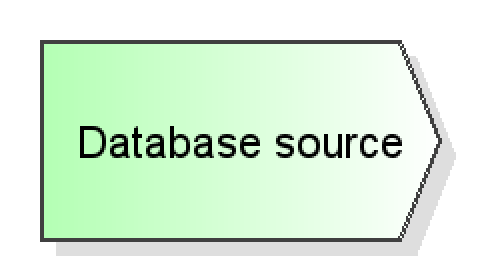
\includegraphics[width=2cm]{imageModelElementSourceDB.png}
\vspace{-22pt}
\end{wrapfigure}

The client source represents the starting point of the movement of a client through the system.
A simulation model can consist of one or more source elements.
At a table-based source clients are not created based on inter-arrival times but the
times are loaded from a database table.

\subsection*{Settings}

The name of the database source element has no meaning for the simulation.
At each database source next to the database connection settings the
name of a database table from which the arrivals are to be loaded and
the names of the row containing the arrival times (in seconds), the
corresponding client types and optional a column for additional client
data have to be specified. Additional the names of the client types
which are to be respected when loading the database table have to
be specified.

The client data column has to contain expressions of the form 
"\texttt{ClientData(1)=5}", "\texttt{ClientData('key')=TextValue}"
or \texttt{w=Formula}. (Instead of \texttt{w} also \texttt{t}, \texttt{p},
\texttt{wCosts}, \texttt{tCosts} and \texttt{pCosts} are available.)
If multiple assignments are to be made for an arriving client
the expressions can be split by \textbf{tabs} in the cell.


\section{Excel DDE source}
\label{ref:ModelElementSourceDDE}

\begin{wrapfigure}{l}{2.5cm}
\vspace{-22pt}
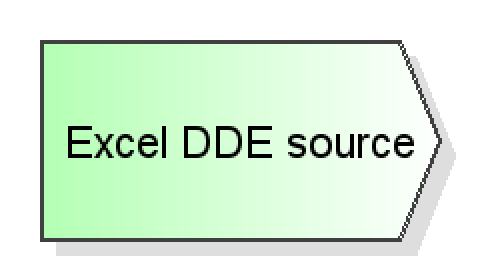
\includegraphics[width=2cm]{imageModelElementSourceDDE.png}
\vspace{-22pt}
\end{wrapfigure}

The client source represents the starting point of the movement of a client through the system.
A simulation model can consist of one or more source elements.
At a DDE table-based source clients are not created based on inter-arrival times but the
times are loaded via DDE from a table.

\subsection*{Settings}

The name of the Excel DDE source element has no meaning for the simulation.
At a Excel DDE source the \textbf{DDE connection settings}
(workbook, table, starting cell) via which the arrivals are to be loaded and the
\textbf{list of the client types} for which client
arrivals are to be loaded from the table have to be specified.

\textbf{Format of the table:}~\\
Tables to be used at a Excel DDE source element have to consist of at least two columns.
The first column has to contain the time stamps of the individual client arrivals
or the inter-arrival times. The values represent the number of seconds since the
start of the simulation or since the last client arrival.
In the second column the client type names of clients which arrive at the times
noted in the first column are defined. Rows containing a client type which is
not in the client types list in the table source element are ignored.
All optional further columns have to contain expressions of the form
\texttt{ClientData(nr)=Formula}, \texttt{ClientData('key')=TextValue},
\texttt{w=Formula}, \texttt{t=Formula}, \texttt{p=Formula},
\texttt{wCosts=Formula}, \texttt{tCosts=Formula} or \texttt{pCosts=Formula}.
Using these expression new client objects can get client-specific data directly.


\section{Exit}
\label{ref:ModelElementDispose}

\begin{wrapfigure}{l}{2.5cm}
\vspace{-22pt}
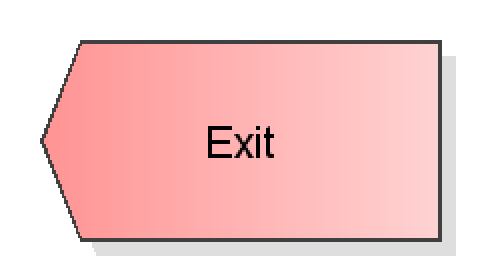
\includegraphics[width=2cm]{imageModelElementDispose.png}
\vspace{-22pt}
\end{wrapfigure}

Any number of edges can be inserted into an exit element, but no edges run out of this element.
The exit represents the last station of a client in the queue system.
At this station, the client leaves the system, and no further processing is possible thereafter.
All the ways of the client have to end in such an element.

\subsection*{Settings}

The name of the exit element has no further meaning for the simulation.

The exit element can be defined as an emergency exit: In this mode, the simulation is aborted
as soon as a client arrives at the station.


\section{Multi source}
\label{ref:ModelElementSourceMulti}

\begin{wrapfigure}{l}{2.5cm}
\vspace{-22pt}
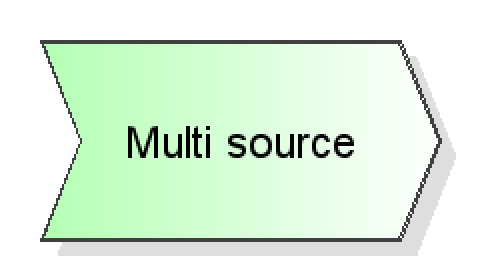
\includegraphics[width=2cm]{imageModelElementSourceMulti.png}
\vspace{-22pt}
\end{wrapfigure}

The multi source represents the starting point of the movement of a client through the system.
A simulation model can consist of one or more source or multi source elements.

\subsection*{Settings}

The name of the multi source element has no meaning for the simulation.

Per individual sub source the following settings can be made:

Per sub source a \textbf{name} for the client type of the clients to be generated has to be defined.
The dialog consists of a number of tabs which allow to setup the different properties of the client source:

\subsubsection*{Inter-arrival time}

With respect to the inter-arrival times, it is possible to determine whether these
should be determined according to a \textbf{distribution}, according to an \textbf{expression},
on a \textbf{schedule} or by a \textbf{release condition}, a \textbf{threshold value} or by
one or multiple \textbf{signals}.

\subsubsection*{Batch size}

A batch size larger than 1 can be used to specify that, per arrival, not a single client,
but several clients should arrive at the same time. It is possible to set up the same number
of clients per arrival (fixed batch size) or a distribution of the rates according to which
the respective sizes of the arrival batches are to be determined.
In case of batch arrivals, the inter-arrival times refer to the distances from one batch to the next.
If, for example, batches of each 3 clients arrive with an average inter-arrival time of 2 minutes,
one client arrives every 40 seconds on average.

\subsubsection*{Number of arrivals}

In the general case, a source element generates constantly arrivals according to the
inter-arrival time distribution until the total number of clients in the simulation has been reached
or the simulation has been terminated by an expression. But it can also be defined that the
source element stops generating clients after a specified number of clients.
Alternatively, a maximum number of clients to be generated can be specified.
If no batch arrivals are used, the number of arrival events equals the
number of clients. For batch arrivals, more clients will arrive than there are arrival events.

\subsubsection*{Starting time}

In the default case the source elements starts generating arrivals immediately after
starting the simulation. By defining some other start time the client generation
(e.g. the first inter-arrival time before the first client arrival) will start at a later
point of time.

\subsubsection*{Assignment of client variables}

On this tab client variable assignment to variables like \texttt{ClientData(nr)} can be setup.
These assignments are applied to each client created by this source.

\subsubsection*{Assignment of texts}

On this tab client text assignments like key:=value can be setup.
These assignments are applied to each client created by this source.


\section{Save and exit}
\label{ref:ModelElementDisposeWithTable}

\begin{wrapfigure}{l}{2.5cm}
\vspace{-22pt}
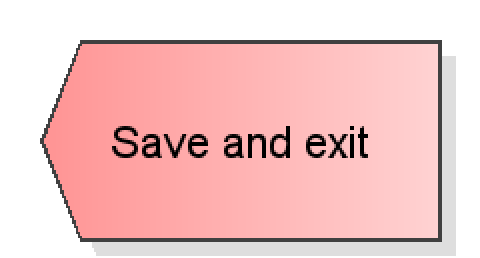
\includegraphics[width=2cm]{imageModelElementDisposeWithTable.png}
\vspace{-22pt}
\end{wrapfigure}

Any number of edges can be inserted into an exit element, but no edges run out of this element.
The exit represents the last station of a client in the queue system.
At this station, the client leaves the system, and no further processing is possible thereafter.
All the ways of the client have to end in such an element.

A Save and exit element stores the data of the individual clients in a table before they leave the system.
Tables generated in this way can be used at table sources (see page \pageref{ref:ModelElementSourceTable}) stations
to use the clients who left the current system as an input stream in another model.

\subsection*{Settings}

For a Save and exit element, a file must be specified where clients are to be recorded before leaving the system.

The name of the exit element has no further meaning for the simulation.

The exit element can be defined as an emergency exit: In this mode, the simulation is aborted
as soon as a client arrives at the station.


\section{Source}
\label{ref:ModelElementSource}

\begin{wrapfigure}{l}{2.5cm}
\vspace{-22pt}
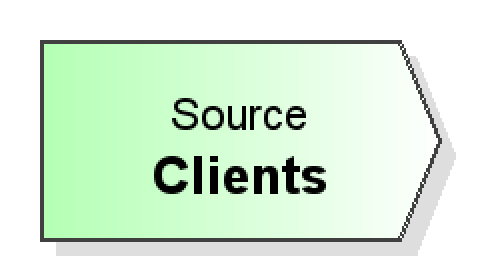
\includegraphics[width=2cm]{imageModelElementSource.png}
\vspace{-22pt}
\end{wrapfigure}

The client source represents the starting point of the movement of a client through the system.
A simulation model can consist of one or more source elements.

\subsection*{Settings}

The \textbf{name} of the source element also defines the names of the clients who originate from it.
The dialog consists of a number of tabs which allow to setup the different properties of the client source:

\subsubsection*{Inter-arrival time}

With respect to the inter-arrival times, it is possible to determine whether these
should be determined according to a \textbf{distribution}, according to an \textbf{expression},
on a \textbf{schedule} or by a \textbf{release condition}, a \textbf{threshold value} or by
one or multiple \textbf{signals}.

\subsubsection*{Batch size}

A batch size larger than 1 can be used to specify that, per arrival, not a single client,
but several clients should arrive at the same time. It is possible to set up the same number
of clients per arrival (fixed batch size) or a distribution of the rates according to which
the respective sizes of the arrival batches are to be determined.
In case of batch arrivals, the inter-arrival times refer to the distances from one batch to the next.
If, for example, batches of each 3 clients arrive with an average inter-arrival time of 2 minutes,
one client arrives every 40 seconds on average.

\subsubsection*{Number of arrivals}

In the general case, a source element generates constantly arrivals according to the
inter-arrival time distribution until the total number of clients in the simulation has been reached
or the simulation has been terminated by an expression. But it can also be defined that the
source element stops generating clients after a specified number of clients.
Alternatively, a maximum number of clients to be generated can be specified.
If no batch arrivals are used, the number of arrival events equals the
number of clients. For batch arrivals, more clients will arrive than there are arrival events.

\subsubsection*{Starting time}

In the default case the source elements starts generating arrivals immediately after
starting the simulation. By defining some other start time the client generation
(e.g. the first inter-arrival time before the first client arrival) will start at a later
point of time.

\subsubsection*{Assignment of client variables}

On this tab client variable assignment to variables like \texttt{ClientData(nr)} can be setup.
These assignments are applied to each client created by this source.

\subsubsection*{Assignment of texts}

On this tab client text assignments like key:=value can be setup.
These assignments are applied to each client created by this source.


\section{Table source}
\label{ref:ModelElementSourceTable}

\begin{wrapfigure}{l}{2.5cm}
\vspace{-22pt}
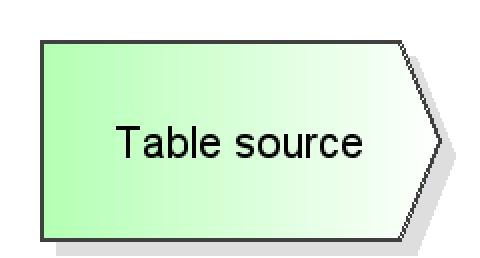
\includegraphics[width=2cm]{imageModelElementSourceTable.png}
\vspace{-22pt}
\end{wrapfigure}

The client source represents the starting point of the movement of a client through the system.
A simulation model can consist of one or more source elements.
At a table-based source clients are not created based on inter-arrival times but the
times are loaded from a table.

\subsection*{Settings}

The name of the table source element has no meaning for the simulation.
At a table source the \textbf{file name of the table} from which the arrivals
are to be loaded and the \textbf{list of the client types} for which client
arrivals are to be loaded from the table have to be specified.

\textbf{Format of the table:}~\\
Tables to be used at a table source element have to consist of at least two columns.
The first column has to contain the time stamps of the individual client arrivals
or the inter-arrival times. The values represent the number of seconds since the
start of the simulation or since the last client arrival.
In the second column the client type names of clients which arrive at the times
noted in the first column are defined. Rows containing a client type which is
not in the client types list in the table source element are ignored.
All optional further columns have to contain expressions of the form
\texttt{ClientData(nr)=Formula}, \texttt{ClientData('key')=TextValue},
\texttt{w=Formula}, \texttt{t=Formula}, \texttt{p=Formula},
\texttt{wCosts=Formula}, \texttt{tCosts=Formula} or \texttt{pCosts=Formula}.
Using these expression new client objects can get client-specific data directly.

\textbf{Hint:}
The button to the right of the table file input line can be used to open the 
Prepare table for table source dialog,
where tables in normal column form can be converted to tables in the format described above.





\chapter{Processing}

\section{Delay}
\label{ref:ModelElementDelay}

\begin{wrapfigure}{l}{2.5cm}
\vspace{-22pt}
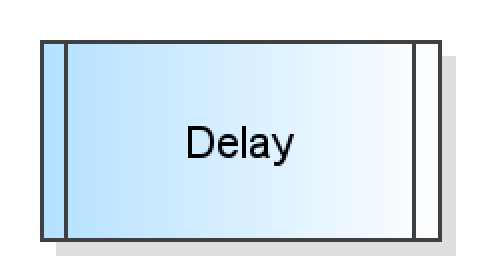
\includegraphics[width=2cm]{imageModelElementDelay.png}
\vspace{-22pt}
\end{wrapfigure}

When passing a delay element, the clients are delayed for a specific time period which can be determined
 by means of a distribution function or an expression. There will be no further processing on the clients.

\subsection*{Settings}

The name of the delay element has no further meaning. The distribution or the expression of the delay times can be used
to determine how long the individual clients have to wait while passing the element. A global distribution or expression,
which is always applied when no client-type-specific data are defined, and optionally an individual distribution or expression
can be specified for each client type.

If clients are to be released via an external script element for further movement through the system before the delay time has elapsed,
it must be activated via the corresponding checkbox that a corresponding list for script access should be provided. The provision of
this list slows down the simulation, even if it is not accessed.


\section{Process station}
\label{ref:ModelElementProcess}

\begin{wrapfigure}{l}{2.5cm}
\vspace{-22pt}
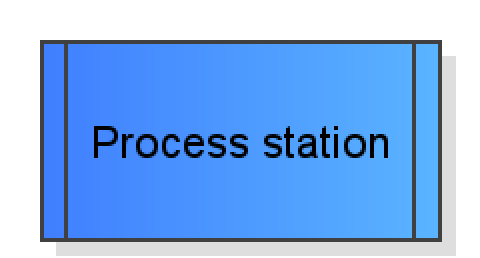
\includegraphics[width=2cm]{imageModelElementProcess.png}
\vspace{-22pt}
\end{wrapfigure}

The process station is the central element of each simulation model. In an process station, clients wait for an operator
to become available and then are served by this operator for a certain time. Clients whose (optional) limited waiting time
tolerance has been exceeded will cancel waiting without having been served. An operator (also optionally) can go into
a post-processing time after serving a client, before he is again ready to serve the next client.

It can be stated that, instead of one operator, several operators are optionally required from several different groups
to serve a client.

Additionally it can also be set up that clients are not served individually, but in groups.
In this case, the necessary numbers of operators refer to operating a whole group.

\subsection*{Settings}

\subsubsection*{Name}

The name of the process station element has no further meaning.

\subsubsection*{Processing times}

On this dialog page, the probability distribution or the expression for the clients's processing times can be set.
Optionally, an individual distribution or expressions can be defined for each client type.

\textbf{Note on individual processing times and batch processing:}~\\
In principle, individual client processing times and the simultaneous operation of several clients
(of possibly different types) contradict each. Nevertheless, this can be used in the simulation.
In this case, an processing time according to the predefined distribution is determined for each
client type contained in the batch. This processing time then applies to all clients in the batch
of client's type. The resources are seized until the maximum of the processing times for all
clients included in the batch is reached.

\subsubsection*{Setup times}

On this dialog page, additional times between the service processes of clients of the same
or - which is usually the case - of different types can be defined. These setup times,
which are optional for each client type transition, can be defined each using either a
probability distribution or an expression.

\textbf{Note on setup times and batch processing:}~\\
Setup times and batching cannot be used at the same time at one process station.
A process station with setup times can serve clients which are temporary or
permanently batched but creating batches directly at the process station is
not possible in this case, because the simulator would not be able to determine
which setup time is in charge in this case.

\subsubsection*{Post processing times}

The optional post-processing times can be used to specify a probability distribution or an expression
according to which the operator will require additional time after the client has been served before they are
available to process the next client. Optionally, an individual distribution can also be set
for each client type.

\textbf{Note about individual post-processing times and batch processing:}~\\
In principle, individual client post-processing times and the simultaneous operation of several clients
(of possibly different types) contradict each. Nevertheless, this can be used in the simulation.
In this case, an post-processing time according to the predefined distribution is determined for each
client type contained in the batch. The resources are seized until the maximum of the post-processing times
for all clients included in the batch is reached.

\subsubsection*{Waiting time tolerances}

If the clients are only willing to wait for a limited period of time, a waiting time tolerance (based on a distribution
or on an expression) is determined for each client according to the waiting time tolerance distribution
(globally or optionally individual per client type). If this time is exceeded, the client cancels waiting and leaves
the system without being served.

\subsubsection*{Priorities and batch sizes}

If more than one client is waiting and an operator is available, the client to be served next is determined by the 
priorities. The client with the highest priority will be served next. 
"w" indicates here the client's previous waiting time at the current station. (In all other cases "w" is the total
waiting time of the current client.) This means that the formula "w" for the priority results
in a first-in-first-out queue. "-w" would result in a last-in-first-out system.
The batch size indicates how many clients can be operated simultaneously by an operator. Obviously, the minimum batch
size can not be larger as the maximum batch size. If both values are identical, a fixed batch size is obtained.
If the minimum batch size is actually smaller than the maximum batch size, after waiting for this minimum number of
waiting customers, a millisecond is still waited to see if further customers arrive. Then at least as many clients
as before (= minimum batch size) and at most as many of the waiting clients as the maximum batch size are served.

\textbf{Note about variable batch sizes in the simulation:}~\\
Clients are basically moving through the queueing network as individual objects.
As a result, when a variable batch size is used, the client group operation would theoretically always
start with the minimum batch size. - Even if the next client of the virtual batch would arrive immediately.
In order to accommodate this fact, the simulator waits a millisecond after the arrival of a client, which
increases the number of waiting clients to the minimum necessary batch size, so as to allow the addition
of further directly incoming clients to the batch.

\subsubsection*{Operators}

To operate a client (or a client batch) several operators from several groups can be required.
The operation starts only if all necessary operators are available at the same time and all can be seized
simultaneously.
Additionally alternative group setups can be defined. All groups of one setup have to be available in order
to start the service of a client. The alternatives will be checked for availability in the defined order.

The resource priority can be used to determine the priority of this process station when a resource
which is necessary for processing the clients at this station becomes free. Larger values mean a
higher priority, or a higher probability, that this process station gets the appropriate resources
if there are multiple process stations that need the same resource.

\subsubsection*{Costs}

On this page, you can optionally set the costs incurred by the clients. This are costs of the process station.
For the waiting, transfer and operating times costs per client can be defined in the clients settings for each
client type. Also the costs for allocation and availability of the resources can be defined in the resource settings.





\chapter{Assignments}

\section{Assign string}
\label{ref:ModelElementAssignString}

\begin{wrapfigure}{l}{2.5cm}
\vspace{-22pt}
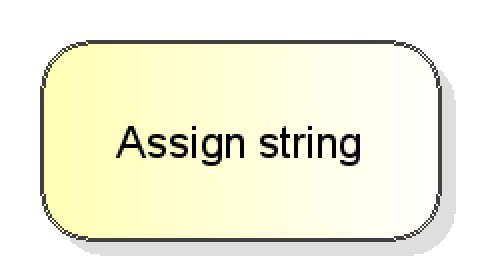
\includegraphics[width=2cm]{imageModelElementAssignString.png}
\vspace{-22pt}
\end{wrapfigure}

The assign string element assigns one or more text values to keys of all clients passing this element.

\subsection*{Settings}

The name of the type assign string element has no further meaning for the simulation.
For each assignment a non-empty key has to be choosen. The value can optionally be an empty string.


\section{Batch counter}
\label{ref:ModelElementCounterBatch}

\begin{wrapfigure}{l}{2.5cm}
\vspace{-22pt}
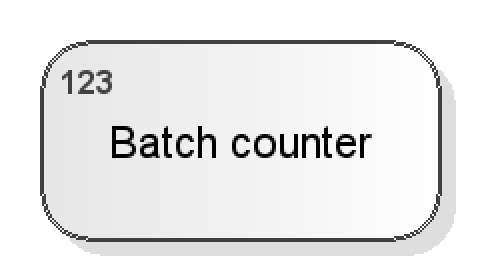
\includegraphics[width=2cm]{imageModelElementCounterBatch.png}
\vspace{-22pt}
\end{wrapfigure}

If clients pass through this station with a time interval of 0 seconds, they are counted as a batch.
The counting is done on a batch basis as well as differentiated by batch sizes.

\subsection*{Settings}

The counter name defines the name under which the results are to be recorded in the statistics.


\section{Client statistics}
\label{ref:ModelElementSetStatisticsMode}

\begin{wrapfigure}{l}{2.5cm}
\vspace{-22pt}
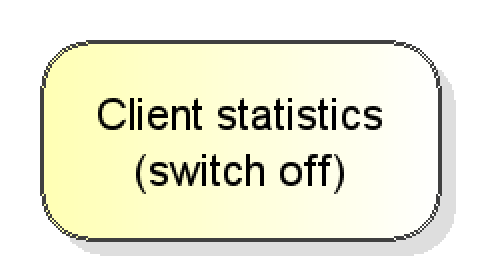
\includegraphics[width=2cm]{imageModelElementSetStatisticsMode.png}
\vspace{-22pt}
\end{wrapfigure}

The client statistics elements allows to switch statistics recording
for the current client on or off.

\subsection*{Settings}

The name of the client statistics element has no further meaning.
In the element has to be set up if the recording is to be switch on or off
for the clients passing this element.


\section{Costs}
\label{ref:ModelElementCosts}

\begin{wrapfigure}{l}{2.5cm}
\vspace{-22pt}
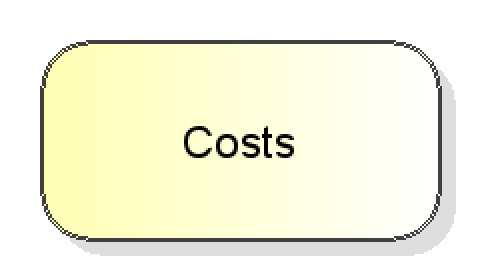
\includegraphics[width=2cm]{imageModelElementCosts.png}
\vspace{-22pt}
\end{wrapfigure}

If a client passes this element, some waiting, transfer and process time costs can be added to the
statistics. In addition, costs due to the station itself can be recorded, too.

\subsection*{Settings}

The name of the cost element has no further meaning. The defined clients costs are recorded in the clients element
of the client who passes the station. Additionally, costs can be specified which are recorded for the station itself.


\section{Counter}
\label{ref:ModelElementCounter}

\begin{wrapfigure}{l}{2.5cm}
\vspace{-22pt}
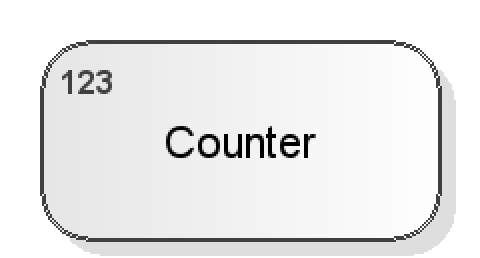
\includegraphics[width=2cm]{imageModelElementCounter.png}
\vspace{-22pt}
\end{wrapfigure}

If a client passes through this element, the associated counter is incremented by one.
In this way, it is possible to measure how many clients have chosen a specific path in the simulation model.

\subsection*{Settings}

In addition to the name of the counter, a group name for the counter has also to be specified.
Next to the respective absolute value, the proportion of the counter within its respective group
will be indicated in the statistics.


\section{Difference counter}
\label{ref:ModelElementDifferentialCounter}

\begin{wrapfigure}{l}{2.5cm}
\vspace{-22pt}
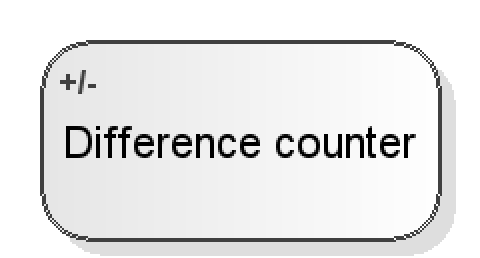
\includegraphics[width=2cm]{imageModelElementDifferentialCounter.png}
\vspace{-22pt}
\end{wrapfigure}

If a client passes through this element, the associated counter is increased or decreased by a certain value.
The minimum value of the counter is 0. If several difference counters have the same name, they share the same
counter object.

\subsection*{Settings}

The name of the element specifies the counter object, which is to be changed by the element by the specified value
when a client passes the element. The minimum and, at the same time, start value of each counter is 0.


\section{Enter section}
\label{ref:ModelElementSectionStart}

\begin{wrapfigure}{l}{2.5cm}
\vspace{-22pt}
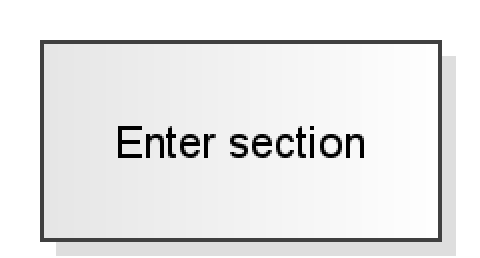
\includegraphics[width=2cm]{imageModelElementSectionStart.png}
\vspace{-22pt}
\end{wrapfigure}

By using sections the residence time of a client in some segment of the model can be measured.
A client passing through this station is immediately forwarded to the next station.
However, leaving the station is not recorded in the station statistics, so from the station
statistics point of view the client is still at this station. Only when the client moves through
an appropriate Leave section element (see page \pageref{ref:ModelElementSectionEnd}) it will be
virtually removed from the station.

\subsection*{Settings}

Stations of this type must have a name which allows them to be addressed by
Leave section elements (see page \pageref{ref:ModelElementSectionEnd}) to signal
that the client has now left the section.


\section{Leave section}
\label{ref:ModelElementSectionEnd}

\begin{wrapfigure}{l}{2.5cm}
\vspace{-22pt}
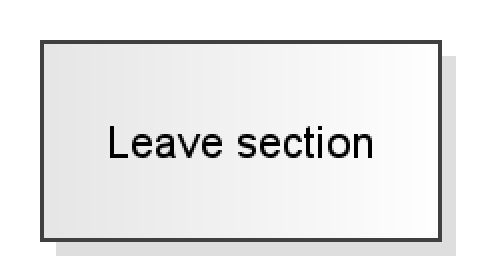
\includegraphics[width=2cm]{imageModelElementSectionEnd.png}
\vspace{-22pt}
\end{wrapfigure}

By using a Leave section element, an Enter section element (see page \pageref{ref:ModelElementSectionStart}) 
can be told that a client has left the model segment under consideration.

\subsection*{Settings}

The name of the Leave section element has no further meaning for the simulation.
The name of the Enter section (see page \pageref{ref:ModelElementSectionStart}) station
from which the client should be discharged while passing through this element has
to be specified. If the client has not passed the associated
Enter section element (see page \pageref{ref:ModelElementSectionStart}) before,
no processing will occur.


\section{Multi counter}
\label{ref:ModelElementCounterMulti}

\begin{wrapfigure}{l}{2.5cm}
\vspace{-22pt}
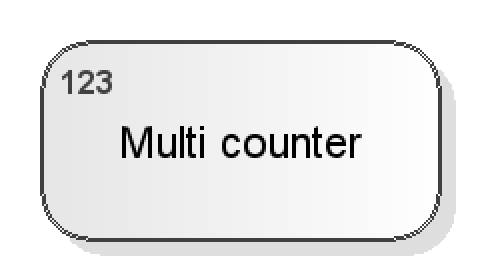
\includegraphics[width=2cm]{imageModelElementCounterMulti.png}
\vspace{-22pt}
\end{wrapfigure}

If a client passes through this element, depending on different conditions the value
of one counter is incremented by one. In this way, it is possible to measure how many
clients have chosen a specific path in the simulation model. A multi counter works
like a decision (see page \pageref{ref:ModelElementDecide}) by expression element followed
by some normal counter elements (see page \pageref{ref:ModelElementCounter}) .

\subsection*{Settings}

The name of the multi counter element has no meaning for the simulation. By choosing
a common group name for the counters in the statistics not only the absolute values
of the counters will be reported but also the relative part of each counter in its
group. If a client passes through this element, the given expressions will be checked
one after each other. The value of the counter for the first fullfilled condition will
be increased by one. If non of the conditions it met, the counter for the "else" case
will be increased.


\section{Script}
\label{ref:ModelElementSetJS}

\begin{wrapfigure}{l}{2.5cm}
\vspace{-22pt}
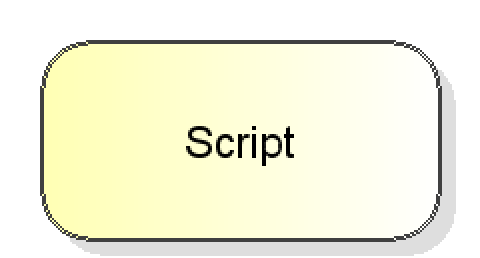
\includegraphics[width=2cm]{imageModelElementSetJS.png}
\vspace{-22pt}
\end{wrapfigure}

If a client passes through this element, variable assignments defined via
a Javascript or Java programm are executed.

\subsection*{Settings}

The name of the Script element has no further meaning.
The script commands to be executed are defined in \textbf{Javascript} or \textbf{Java}.
Next to the default Javascript or Java commands some additional Javascript commands 
or additional Java commands are available for accessing the simulation data.

\subsection*{Alternative}

The Javascript or Java based variable assignment allows maximum flexibility, but takes a comparatively long
computing time. A faster option for assigning variables is using the
Variable element (see page \pageref{ref:ModelElementSet}) .


\section{State}
\label{ref:ModelElementStateStatistics}

\begin{wrapfigure}{l}{2.5cm}
\vspace{-22pt}
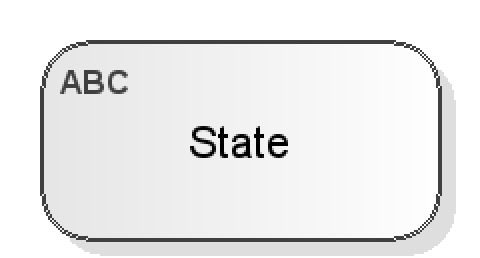
\includegraphics[width=2cm]{imageModelElementStateStatistics.png}
\vspace{-22pt}
\end{wrapfigure}

If a client passes through this element, the associated system state is set in the statistics.
By using multiple state statistics elements it can be recorded how long the system
was in which state.

\subsection*{Settings}

In addition to the name of the element, a group name for the state has also to be specified.
Next to the respective absolute value, the proportion of time the system was in the specified
state according to all states om the group will be indicated in the statistics.


\section{Throughput}
\label{ref:ModelElementThroughput}

\begin{wrapfigure}{l}{2.5cm}
\vspace{-22pt}
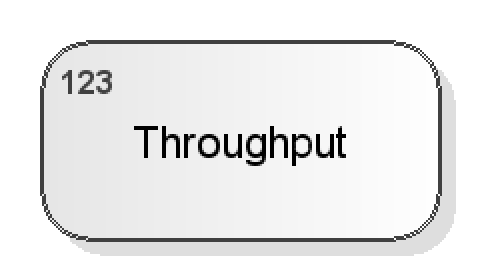
\includegraphics[width=2cm]{imageModelElementThroughput.png}
\vspace{-22pt}
\end{wrapfigure}

If a client passes through this element, the associated counter is incremented by one
and the current time is recorded. In this way, it is possible to measure the client
throughput per time unit through this element.

\subsection*{Settings}

The name of the throughput element has no further meaning for the simulation itself.
But a name has to be specified for the element because the measured throughput is
displayed using this name in the statistics.


\section{Type assignment}
\label{ref:ModelElementAssign}

\begin{wrapfigure}{l}{2.5cm}
\vspace{-22pt}
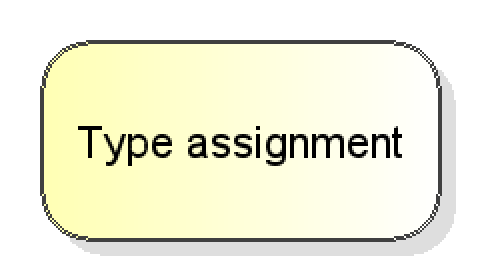
\includegraphics[width=2cm]{imageModelElementAssign.png}
\vspace{-22pt}
\end{wrapfigure}

The type assignment element assigns a new client type (for the statistics) to the clients who are passing this element.

\subsection*{Settings}

The name of the type assignment element is at the same time the client type that all clients who pass through this element receive.


\section{Variable}
\label{ref:ModelElementSet}

\begin{wrapfigure}{l}{2.5cm}
\vspace{-22pt}
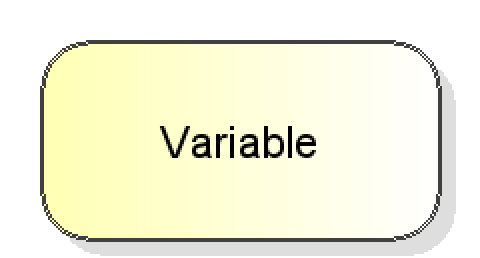
\includegraphics[width=2cm]{imageModelElementSet.png}
\vspace{-22pt}
\end{wrapfigure}

If a client passes through this element, the variable assignments defined in
this element are executed. In all other elements in which expressions are evaluated,
especially in the Condition element (see page \pageref{ref:ModelElementHold}) , these variables can be accessed.

Initial all variables are set to 0. By using assignments like \texttt{a:=a+1} counters can be realized.

\subsection*{Settings}

The name of the variable element has no further meaning.
The assignments are processed in the order in which they are defined in the element when a client passes the element.

By using the pseudo variables "w", "t" and "p" you can access the waiting time, the transfer time and the
process time of the current client (each on second base) for reading and for writing. Additionally you can
write to a client object data field by using "ClientData(index)" as target variable.

\subsection*{Alternative}

The Javascript element (see page \pageref{ref:ModelElementSetJS}) allows to define more complex assignment.
On the other side the Javascript element will need much more computing time to be executed during simulation.





\chapter{Branching}

\section{Balking}
\label{ref:ModelElementBalking}

\begin{wrapfigure}{l}{2.5cm}
\vspace{-22pt}
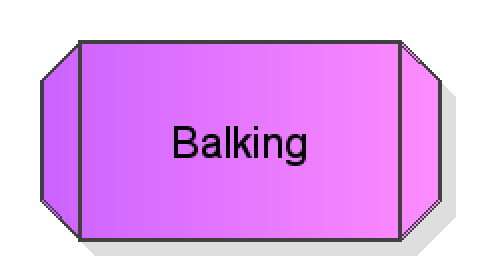
\includegraphics[width=2cm]{imageModelElementBalking.png}
\vspace{-22pt}
\end{wrapfigure}

The Balking element checks if clients are waiting at the next process station reachable
on the direct way. In this case the condition (which may contain random expressions depending
on some client properties) is evaluated. If the condition is true, the client will balk to
enter the queue and leaves the Balking element by the connection which is intended for this
case.

\subsection*{Settings}

The name of the Balking element has no further meaning for the simulation.
The entered expression will be evaluated if there is a queue of waiting
clients on the next process station and determines if the client is willing
to enter the queue or if he is balking to do so. As expression a condition or
a balking probability can be entered. The value can also be set up global or
by client type.


\section{Decide}
\label{ref:ModelElementDecide}

\begin{wrapfigure}{l}{2.5cm}
\vspace{-22pt}
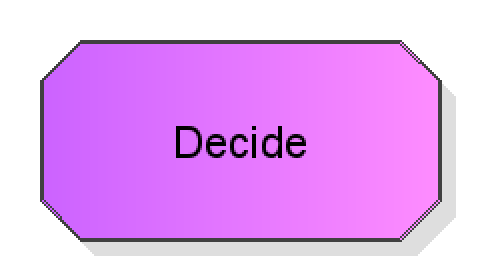
\includegraphics[width=2cm]{imageModelElementDecide.png}
\vspace{-22pt}
\end{wrapfigure}

This element allows to forward the incoming clients to several different possible output directions.
The branching can be carried out according to the following criteria:

\begin{itemize}
  \item 
    \textbf{Random:}
    For each exit direction a rate is specified, which determines the probability for this route.

  \item 
    \textbf{Condition:}
    Conditions are defined for all output directions (except for the last direction).
    If a client arrives, these conditions are checked from top to bottom.
    The client is forwarded in the direction in which the condition was fulfilled for the first time.
    If none of the conditions apply, the customer is forwarded in the last direction
    (for which no condition is specified).

  \item 
    \textbf{Client type:}
    Client types are defined for all output directions (except for the last direction).
    If an arriving client is of one of these types, it is forwarded in the corresponding direction.
    If the type of the arrived client does not correspond to any of the specified client types,
    the client is forwarded in the last direction (for which no client type is specified).

  \item 
    \textbf{Sequence:}
    One of the clients is directed to one of the outputs in sequence. After a client is routed to the last
    connected output, the next client is routed back to the first output.

  \item 
    \textbf{Shortest queue at the next station:}
    Routes the client to the path where the next station
    has the shortest queue. In the case of the same value
    for multiple paths, a random decision will be made.

  \item 
    \textbf{Shortest queue at the next process station:}
    Routes the client to the path where the next process station
    has the shortest queue. Stations between the decide element
    and the process station on the path will be ignored when
    calculating the queue length. In the case of the same value
    for multiple paths, a random decision will be made.

  \item  
    \textbf{Least number of clients at the next station:}
    Routes the client to the path where the next station
    has the least current number of clients. In the case of the same value
    for multiple paths, a random decision will be made.    

  \item 
    \textbf{Least number of clients at the next process station:}
    Routes the client to the path where the next process station
    has the least current number of clients. Stations between the decide element
    and the process station on the path will be ignored when
    calculating the number of clients at the process station.    
    In the case of the same value
    for multiple paths, a random decision will be made.    

  \item 
    \textbf{Text property:}
    Values are defined for all output directions (except for the last direction).
    If some special key of an arriving client has the specified value , the client
    is forwarded in the corresponding direction.
    If the value of the arrived client does not correspond to any of the specified values,
    the client is forwarded in the last direction (for which no value is specified).

\end{itemize}

\subsection*{Settings}

\subsubsection*{Mode "Random"}

The forwarding probabilities in the various possible output directions need not be given in the form
of probabilities which have to sum up to 1, but it is sufficient to specify rates. These rates are
automatically normalized by the program to probabilities. The following prerequisites apply:
The rates may not be negative and at least one of the specified rates has to be greater than 0.

\subsubsection*{Mode "Condition"}

For each existing direction, a condition has to be specified under which the clients are routed in this
direction. The conditions do not have to be mutually exclusive and are tested from top to bottom.
No condition can be specified for the last direction. This direction is selected in the simulation
whenever none of the previous conditions were true.

\subsubsection*{Mode "Client type"}

For each direction, a client type has to be specified whose clients are routed in this direction.
No client type can be specified for the last direction. This direction is selected in the simulation
whenever none of the previous conditions were true.

\subsubsection*{Mode "Text property"}

A clients key from which the values are to be read has to be specified.
Additionally for each direction, a value has to be specified. If the client key has this value the client
is routed in this direction. No value can be specified for the last direction. This direction is selected in the simulation
whenever none of the previous conditions were true.

Additionally client types for each outgoing edges can be
defined which will be assigned to the clients leaving the station.


\section{Decide (Skript)}
\label{ref:ModelElementDecideJS}

\begin{wrapfigure}{l}{2.5cm}
\vspace{-22pt}
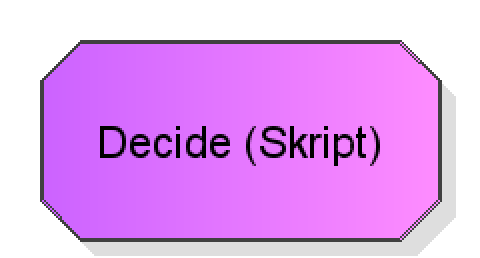
\includegraphics[width=2cm]{imageModelElementDecideJS.png}
\vspace{-22pt}
\end{wrapfigure}

This element allows to forward the incoming clients to several different possible
output directions by using Javascript or Java code.

\subsection*{Settings}

The script code can contain any Javascript or Java commands as well as some
special Javascript commands or
special Java commands for accessing the simulation system.
As return value (to be output by \texttt{Output.print()}) a numerical value
which denotes the exit to choose (1-based) is expected.


\section{Duplicate}
\label{ref:ModelElementDuplicate}

\begin{wrapfigure}{l}{2.5cm}
\vspace{-22pt}
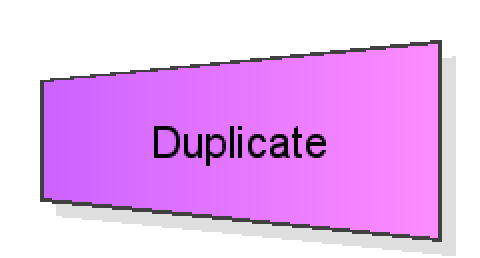
\includegraphics[width=2cm]{imageModelElementDuplicate.png}
\vspace{-22pt}
\end{wrapfigure}

Any number of edges can go into a duplicate element. All client who arrive at the element via these edges are passed on over
the several possible outgoing edges. If several edges run out of the element, the client object is duplicated and a
similar object is passed over each edge.

\subsection*{Settings}

The name of the duplicate element has no further meaning. Additionally client types for each outgoing edges can be
defined which will be assigned to the clients leaving the station.





\chapter{Barriers}

\section{Barrier}
\label{ref:ModelElementBarrier}

\begin{wrapfigure}{l}{2.5cm}
\vspace{-22pt}
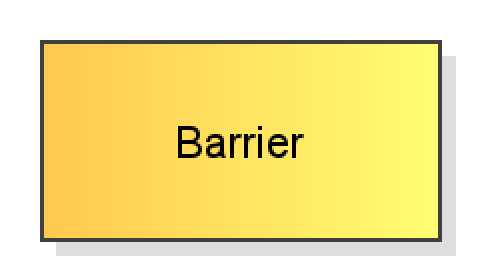
\includegraphics[width=2cm]{imageModelElementBarrier.png}
\vspace{-22pt}
\end{wrapfigure}

This element is used to stop incoming clients until a signal arrives on which they are released.
Corresponding signals are generated if a clients passes a
Signal element (see page \pageref{ref:ModelElementSignal}) .

\subsection*{Settings}

The name of the barrier element has no further meaning. You have to specify a least one
Signal element (see page \pageref{ref:ModelElementSignal}) that signals the release of clients waiting here.
The number of waiting clients which are released at an incoming signal can be set up as well as
if the release should act on all client type or on only one client type.
Furthermore, a number of clients who are allowed to pass the barrier before the counting begins
can be defined.


\section{Condition}
\label{ref:ModelElementHold}

\begin{wrapfigure}{l}{2.5cm}
\vspace{-22pt}
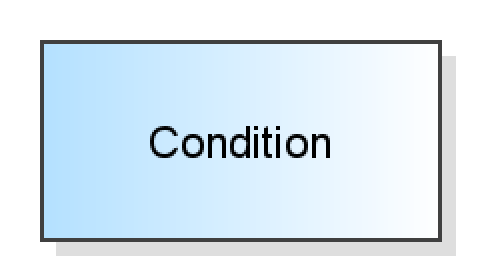
\includegraphics[width=2cm]{imageModelElementHold.png}
\vspace{-22pt}
\end{wrapfigure}

When the condition element is passed, the clients are stopped until the defined condition is fulfilled. 

\subsection*{Settings}

The name of the condition element has no further meaning.
If clients are in the queue, the system checks whether the condition is fulfilled.
If yes, the next client is released. After a (simulation time) millisecond the next check
is performed and, if necessary, the next client is released.
It can be set whether the condition is to be considered globally (without the option of using client-specific variables)
or whether the condition is to be interpreted on a client-specific basis (including the option of using client-specific variables).
In the case of a global interpretation, the condition is evaluated only once; if it is not fulfilled, processing is completed in this step.
In the case of a client-specific interpretation, the condition is evaluated individually for each waiting client in each step (which will take a longer time).
If the condition contains values that can change independently of events (e.g. the simulated time),
it may is necessary, to activate the option "Do additional time-based condition checks". In this case,
the value of the condition is additionally checked in certain time intervals. How long these intervals
are can be configured in the Model properties dialog.
Additional time-based checks significantly slow down the simulation and should only be activated
if this is for the condition necessary.


\section{Condition (Script)}
\label{ref:ModelElementHoldJS}

\begin{wrapfigure}{l}{2.5cm}
\vspace{-22pt}
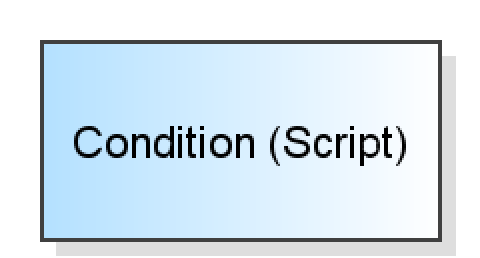
\includegraphics[width=2cm]{imageModelElementHoldJS.png}
\vspace{-22pt}
\end{wrapfigure}

This element allows to hold and forward the incoming clients by using a
Javascript-based or Java-based condition.

\subsection*{Settings}

The script code can contain any Javascript or Java commands as well as some
special Javascript commands or special Java commands 
for accessing the simulation system.

If the condition contains values that can change independently of events (e.g. the simulated time),
it may is necessary, to activate the option "Do additional time-based condition checks". In this case,
the value of the condition is additionally checked in certain time intervals. How long these intervals
are can be configured in the Model properties dialog.
Additional time-based checks significantly slow down the simulation and should only be activated
if this is for the condition necessary.


\section{Multi condition}
\label{ref:ModelElementHoldMulti}

\begin{wrapfigure}{l}{2.5cm}
\vspace{-22pt}
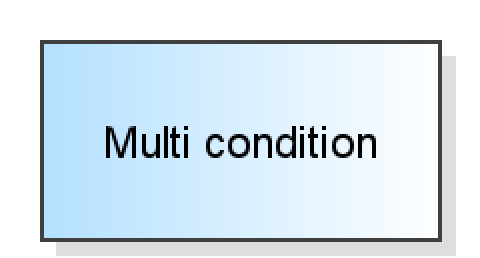
\includegraphics[width=2cm]{imageModelElementHoldMulti.png}
\vspace{-22pt}
\end{wrapfigure}

When a multi condition element is passed, a client ist stopped until for an outgouing edge the
corresponding condition is met. The client is send in the direction where the condition is fulfilled.

\subsection*{Settings}

The name of the multi condition element has no further meaning.
If clients are in the queue, the system checks whether the conditions are fulfilled.
If yes, the next client is released in the direction of the fulfilled condition. After a (simulation time) millisecond the next check
is performed and, if necessary, the next client is released.
If the condition contains values that can change independently of events (e.g. the simulated time),
it may is necessary, to activate the option "Do additional time-based condition checks". In this case,
the value of the condition is additionally checked in certain time intervals. How long these intervals
are can be configured in the Model properties dialog.
Additional time-based checks significantly slow down the simulation and should only be activated
if this is for the condition necessary.


\section{Pull barrier}
\label{ref:ModelElementBarrierPull}

\begin{wrapfigure}{l}{2.5cm}
\vspace{-22pt}
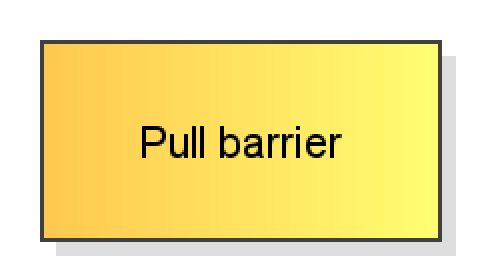
\includegraphics[width=2cm]{imageModelElementBarrierPull.png}
\vspace{-22pt}
\end{wrapfigure}

Pull barriers allow to control the number of clients in some segment.
he pull barrier will only release clients to the next station, if
the total number of clients beginning at this next station to another
(controlled) stations is smaller than a threshold value. This allows to
run some pull effect on the controlled station: If there are
fewer clients at the controlled station than the threshold value allows
at maximum and there are also not enough clients at the next station
following the pull barrier to fill up the queue at the controlled station,
then clients are released from the pull barrier station.

\subsection*{Settings}

The name of the pull barrier element has no further meaning. The name of
the station at which the number of clients is to be controlled has
to be specified and also the maximum number of clients at this controlled
station.


\section{Release resource}
\label{ref:ModelElementRelease}

\begin{wrapfigure}{l}{2.5cm}
\vspace{-22pt}
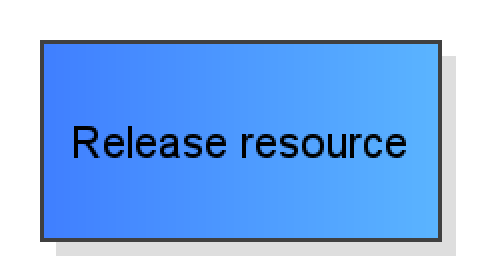
\includegraphics[width=2cm]{imageModelElementRelease.png}
\vspace{-22pt}
\end{wrapfigure}

In a release resource element resources, that have von previously seized by a
Seize resource element (see page \pageref{ref:ModelElementSeize}) , are released again.

The three elements Seize resource (see page \pageref{ref:ModelElementSeize}) , Delay (see page \pageref{ref:ModelElementDelay}) and
\textbf{release resource} in this order therefore work together similar to a
process station element (see page \pageref{ref:ModelElementProcess}) .

\subsection*{Settings}

The name of the release resource element has no further meaning. But it is necessary to specify
which Seize resources (see page \pageref{ref:ModelElementSeize}) should work together with this element.
In addition, a time span can be specified between the arrival of a client at the station and
the release of the resources. If such a time period has been defined, the client will already have
left the release element when the relevant resources are actually released.


\section{Seize resource}
\label{ref:ModelElementSeize}

\begin{wrapfigure}{l}{2.5cm}
\vspace{-22pt}
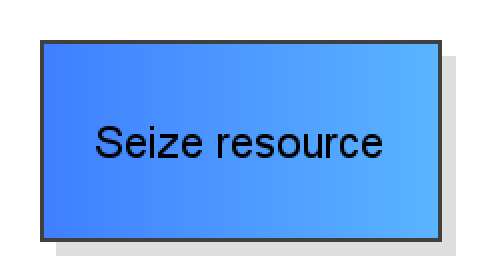
\includegraphics[width=2cm]{imageModelElementSeize.png}
\vspace{-22pt}
\end{wrapfigure}

In order for a client to be able to pass this element, appropriate resources have to be available,
which are seized by the movement of the client through the element but are not released again.

The resources have to be released later by a Release resource element (see page \pageref{ref:ModelElementRelease}) .

The three elements Seize resource (see page \pageref{ref:ModelElementSeize}) , Delay (see page \pageref{ref:ModelElementDelay}) and
\textbf{release resource} in this order therefore work together similar to a
process station element (see page \pageref{ref:ModelElementProcess}) .

\subsection*{Settings}

The seize resource element needs a name because the Release resource elements (see page \pageref{ref:ModelElementRelease}) 
for this resources need to refer to the element.

In order to forward a client may several operators from several groups are required.
The client is only relased if all the necessary operators are available at the same
time and all can be seized simultaneously.

The resource priority can be used to define the priority of this element when a resource that
is necessary at this station becomes free. Larger values mean a higher priority or a higher probability
that this element receives the corresponding resources if there are several stations that need the same resource.


\section{Signal}
\label{ref:ModelElementSignal}

\begin{wrapfigure}{l}{2.5cm}
\vspace{-22pt}
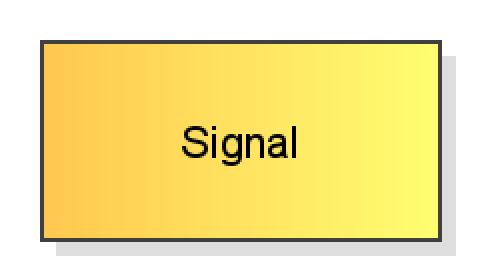
\includegraphics[width=2cm]{imageModelElementSignal.png}
\vspace{-22pt}
\end{wrapfigure}

If a client passes a signal element, the signal corresponding to the name of the element is triggered.
Barrier elements (see page \pageref{ref:ModelElementBarrier}) can be notified by such a signal and can release waiting clients.

\subsection*{Settings}

The name of the signal element is also the name of the signal that is triggered when a client passes the element.





\chapter{Batching}

\section{Batch}
\label{ref:ModelElementBatch}

\begin{wrapfigure}{l}{2.5cm}
\vspace{-22pt}
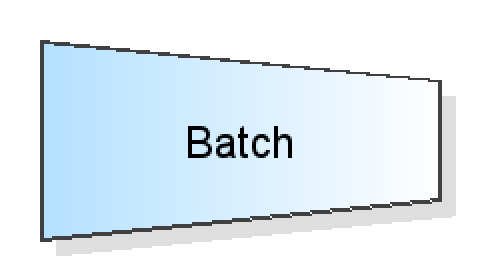
\includegraphics[width=2cm]{imageModelElementBatch.png}
\vspace{-22pt}
\end{wrapfigure}

In this element, incoming clients have to wait until a certain number of clients are available.
These are then forwarded simultaneously or a temporary or a permanent batch is built.

\subsection*{Settings}

The name of the batch element has no further meaning. The minimum and the maximum batch size can be used
to set the number of clients that have to have arrived at minimum at the batch element before they are
forwarded (in batches with maximum the number of specified clients). Furthermore, it can be set whether
the combined clients simply leave the station again (at the same time), or whether a temporary batch (which
can be dissolved by the Dissolve batch element (see page \pageref{ref:ModelElementSeparate}) ) or whether the route
through the network ends for the clients ends at this point (because the two clients, for example, represent
partial components that are combined into a larger element) and instead a new client object is created and
started from this point.


\section{Match}
\label{ref:ModelElementMatch}

\begin{wrapfigure}{l}{2.5cm}
\vspace{-22pt}
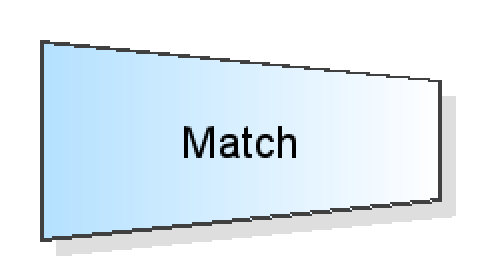
\includegraphics[width=2cm]{imageModelElementMatch.png}
\vspace{-22pt}
\end{wrapfigure}

The match element has two or more inputs. If a client is present at each of the inputs, they are forwarded simultaneously
at the same time or a temporary or a permanent batch is built. If clients are only present at one input line, they have
to wait until clients have also arrived at the other input lines.
In addition, a restriction can be made to only match clients in which a particular client data field has the same
numeric or text value.

\subsection*{Settings}

The name of the match element has no further meaning. For the match element it can be set whether the combined
clients simply leave the station again (at the same time), or whether a temporary batch (which
can be dissolved by the Dissolve batch element (see page \pageref{ref:ModelElementSeparate}) ) or whether the route
through the network ends for the clients ends at this point (because the two clients, for example, represent
partial components that are combined into a larger element) and instead a new client object is created and
started from this point. Additionally a client data field can be defined to be used for matching.


\section{Multi batch}
\label{ref:ModelElementBatchMulti}

\begin{wrapfigure}{l}{2.5cm}
\vspace{-22pt}
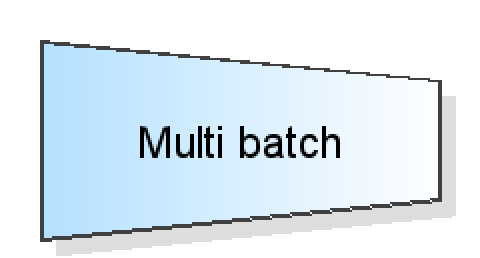
\includegraphics[width=2cm]{imageModelElementBatchMulti.png}
\vspace{-22pt}
\end{wrapfigure}

In this element, incoming clients have to wait until a certain number of clients are available.
These are then forwarded simultaneously or a temporary or a permanent batch is built.
In contrast to the Batch (see page \pageref{ref:ModelElementBatch}) station, you can configure
at this station per client type how many clients are to be combined in which way.

\subsection*{Settings}

The name of the batch element has no further meaning. The minimum and the maximum batch size can be used
to set the number of clients that have to have arrived at minimum at the batch element before they are
forwarded (in batches with maximum the number of specified clients). Furthermore, it can be set whether
the combined clients simply leave the station again (at the same time), or whether a temporary batch (which
can be dissolved by the Dissolve batch element (see page \pageref{ref:ModelElementSeparate}) ) or whether the route
through the network ends for the clients ends at this point (because the two clients, for example, represent
partial components that are combined into a larger element) and instead a new client object is created and
started from this point.
Clients for whose type no batch formation rule is defined will pass the station without further delay.


\section{Pick up}
\label{ref:ModelElementPickUp}

\begin{wrapfigure}{l}{2.5cm}
\vspace{-22pt}
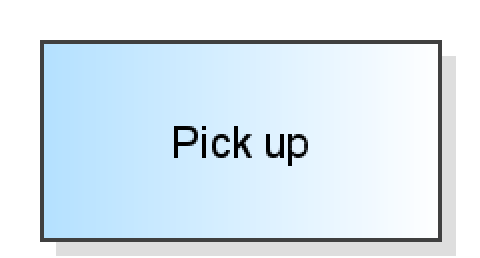
\includegraphics[width=2cm]{imageModelElementPickUp.png}
\vspace{-22pt}
\end{wrapfigure}

If a client passes this element, a client is also taken from the queue of another element and forwarded
along the new path together with the current client or a temporary or a permanent batch is built with the
current client.

\subsection*{Settings}

The name of the pick up element has no further meaning. By specifying a
process station (see page \pageref{ref:ModelElementProcess}) , a condition (see page \pageref{ref:ModelElementHold}) 
or a barrier element (see page \pageref{ref:ModelElementBarrier}) , you can select from which queue the client,
who is to be forwarded together with the current client, should be picked up. You can specify whether
the current client, if there is no client in the queue of the other element, is to be forwarded alone, or
whether the client will wait until another client is present in the other queue. Furthermore, it can be set whether
the combined clients simply leave the station again (at the same time), or whether a temporary batch (which
can be dissolved by the Dissolve batch element (see page \pageref{ref:ModelElementSeparate}) ) or whether the route
through the network ends for the clients ends at this point (because the two clients, for example, represent
partial components that are combined into a larger element) and instead a new client object is created and
started from this point.


\section{Separate}
\label{ref:ModelElementSeparate}

\begin{wrapfigure}{l}{2.5cm}
\vspace{-22pt}
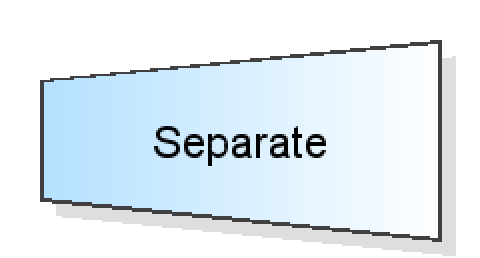
\includegraphics[width=2cm]{imageModelElementSeparate.png}
\vspace{-22pt}
\end{wrapfigure}

If a batch moves through this element, the batch is dissolved into the individual clients from which it is made.
Corresponding batches can be created in the elements Batch (see page \pageref{ref:ModelElementBatch}) ,
Match (see page \pageref{ref:ModelElementMatch}) and Pick up (see page \pageref{ref:ModelElementPickUp}) .

\subsection*{Settings}

The name of the separate element has no further meaning.


\section{Split}
\label{ref:ModelElementSplit}

\begin{wrapfigure}{l}{2.5cm}
\vspace{-22pt}
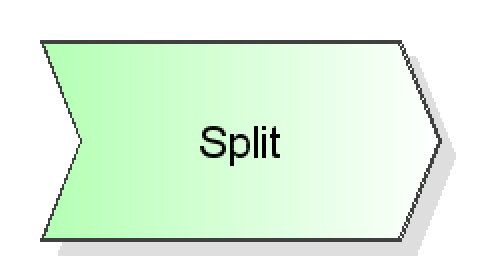
\includegraphics[width=2cm]{imageModelElementSplit.png}
\vspace{-22pt}
\end{wrapfigure}

If a client arrives at a Split station, its live cycle ends there just like
at an  Exit (see page \pageref{ref:ModelElementDispose}) -Element.
Therefore one or more new clients are generated just like at a
einer Multi source element (see page \pageref{ref:ModelElementSourceMulti}) .

\subsection*{Settings}

The name of the split element has no meaning for the simulation.

Per individual sub source the following settings can be made:

Per sub source a \textbf{name} for the client type of the clients to be generated has to be defined.
The dialog consists of a number of tabs which allow to setup the different properties of the client source:

\subsubsection*{Batch size}

A batch size larger than 1 can be used to specify that, per arrival, not a single client,
but several clients should arrive at the same time. It is possible to set up the same number
of clients per arrival (fixed batch size) or a distribution of the rates according to which
the respective sizes of the arrival batches are to be determined.

\subsubsection*{Assignment of client variables}

On this tab client variable assignment to variables like \texttt{ClientData(nr)} can be setup.
These assignments are applied to each client created by this source.

\subsubsection*{Assignment of texts}

On this tab client text assignments like key:=value can be setup.
These assignments are applied to each client created by this source.

\subsubsection*{Transfer of client data from the source client}

Independently of the settings per partial sub source, it is possible to set that
the numeric and text-based client data should be transferred from the source client
to the newly generated clients.





\chapter{Transport}

\section{Assign sequence}
\label{ref:ModelElementAssignSequence}

\begin{wrapfigure}{l}{2.5cm}
\vspace{-22pt}
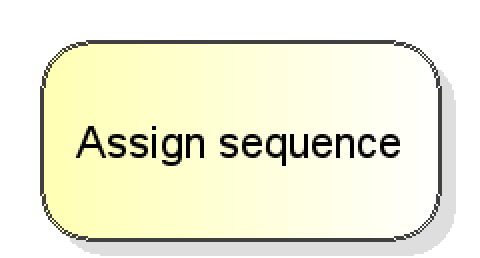
\includegraphics[width=2cm]{imageModelElementAssignSequence.png}
\vspace{-22pt}
\end{wrapfigure}

The assign sequence element assigns a the to the clients who are passing this element an production planning
sequence. The sequence is used at the Transport origin (see page \pageref{ref:ModelElementTransportSource}) 
elements to determine the transport destination of the clients.

\subsection*{Settings}

The name of the assign sequence element has no further meaning. However, a production plan sequence
has to be selected which is assigned to the clients who pass this element.


\section{Conveyor}
\label{ref:ModelElementConveyor}

\begin{wrapfigure}{l}{2.5cm}
\vspace{-22pt}
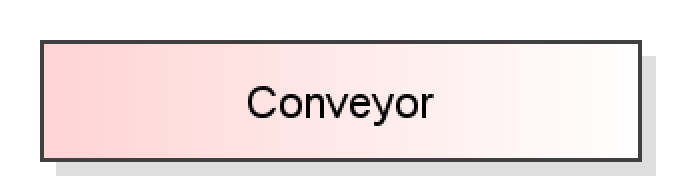
\includegraphics[width=2cm]{imageModelElementConveyor.png}
\vspace{-22pt}
\end{wrapfigure}

A conveyor delays all arriving clients for a fixed time.
Additionally a conveyor has a limited capacity and each
arriving client can need a different amount of this capacity.
Clients for which there is not enough free transport capacity
will need to wait in a queue.

\subsection*{Settings}

The name of the conveyor element has no further meaning for the simulation.
For each conveyor an available transport capacity and a needed capacity for
transporting a single client (optional per client type) can be defined.
Transporting a client along the conveyor will take some defineable fixed
time. This means a client cannot overtake another client on the conveyor.
Additionally the movement direction of the clients on the conveyor during
the animation can be set up.


\section{Parking lot}
\label{ref:ModelElementTransportParking}

\begin{wrapfigure}{l}{2.5cm}
\vspace{-22pt}
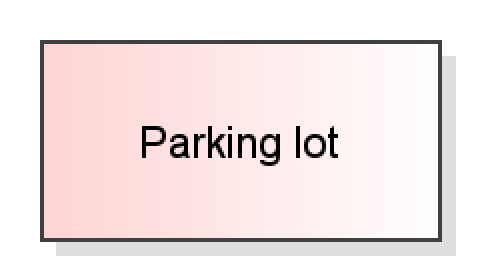
\includegraphics[width=2cm]{imageModelElementTransportParking.png}
\vspace{-22pt}
\end{wrapfigure}

If there is no station requesting a transporter after it has reached its
destination station the transporter will stay at the destination station. 
If the transporter is requested later it will may have to move a far distance
to the requsting origin station. A parking lot station can requst a transporter
just like a origin station. But the transporter will not be loaded at a parking lot;
it will just stay there and wait. The advantage of using parking lots is that
a parking lot can be much closer to a origin station. So if a transporter
already waiting at a parking lot is requested by an origin station the
travel distance may be much shorter.

\subsection*{Settings}

The name of the parking lot element has no further meaning.
The \textbf{Transporter type} drop down box allows to define which
type of transporters is to be attracted by the parking lot station.
The \textbf{Parking lot capacity} defined the maximum number of
transporters which can wait at the station. The
\textbf{Priority for requesting free transporters} should always be
smaller than the priority for requesting free transporters of
origin stations. Otherwise free transporters will head to parking
lots instead of moving to origin stations where they are needed
for transporting.


\section{Teleport transport destination}
\label{ref:ModelElementTeleportDestination}

\begin{wrapfigure}{l}{2.5cm}
\vspace{-22pt}
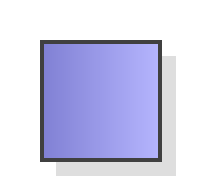
\includegraphics[width=2cm]{imageModelElementTeleportDestination.png}
\vspace{-22pt}
\end{wrapfigure}

Teleport transports allow to timeless transport a client from a 
teleport transport source (see page \pageref{ref:ModelElementTeleportSource}) 
to a teleport transport destination.
In contrast to normal transports, this is not about modeling a clients's actual transport
(which may takes a certain amount of time and requires some resources), but to keep the model clear.
If a client enters a teleport transport source, he is immediately transported to the specified
teleport transport destination. Start and end points can be located in different places in the model;
unlike a transport over an edge, no connection line between start and finish is drawn.

\subsection*{Settings}

The teleport transport destination elements are identified by their names when transporting
clients from a teleport transport source element to a teleport transport destination element.


\section{Teleport transport source}
\label{ref:ModelElementTeleportSource}

\begin{wrapfigure}{l}{2.5cm}
\vspace{-22pt}
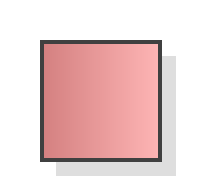
\includegraphics[width=2cm]{imageModelElementTeleportSource.png}
\vspace{-22pt}
\end{wrapfigure}

Teleport transports allow to timeless transport a client from a teleport transport source
to a teleport transport destination (see page \pageref{ref:ModelElementTeleportDestination}) .
In contrast to normal transports, this is not about modeling a clients's actual transport
(which may takes a certain amount of time and requires some resources), but to keep the model clear.
If a client enters a teleport transport source, he is immediately transported to the specified
teleport transport destination. Start and end points can be located in different places in the model;
unlike a transport over an edge, no connection line between start and finish is drawn.

\subsection*{Settings}

The name of the teleport transport source element has no further meaning for the simulation.
However, the name of a Teleport transport destination (see page \pageref{ref:ModelElementTeleportDestination}) 
to which the arriving clients are to be transported has to be specified.


\section{Transport destination}
\label{ref:ModelElementTransportDestination}

\begin{wrapfigure}{l}{2.5cm}
\vspace{-22pt}
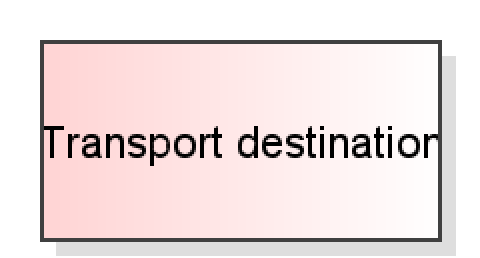
\includegraphics[width=2cm]{imageModelElementTransportDestination.png}
\vspace{-22pt}
\end{wrapfigure}

The transport destination elements can be used a target stations when transporting
clients from a transport origin (see page \pageref{ref:ModelElementTransportSource}) 
element. There is no need for a connection edge between the transport origin element
and the transport destination element for routing clients from the origin to the
destination.

\subsection*{Settings}

The transport destination elements are identified by their names when routing
clients from a transport origin element to a transport destination element.


\section{Transport origin}
\label{ref:ModelElementTransportSource}

\begin{wrapfigure}{l}{2.5cm}
\vspace{-22pt}
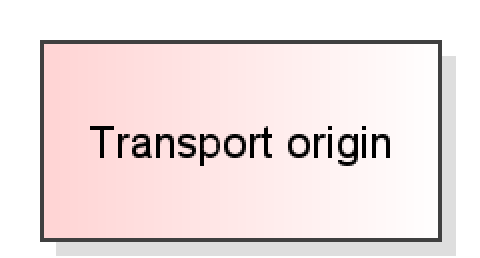
\includegraphics[width=2cm]{imageModelElementTransportSource.png}
\vspace{-22pt}
\end{wrapfigure}

A transport origin element allows to transport a client to any
transport destination (see page \pageref{ref:ModelElementTransportDestination}) 
element. How much time is needed for the transport and to which
transport destination element the client is transported can be set up
in the transport origin element. 
There is no need for a connection edge between the transport origin element
and the transport destination element for routing clients from the origin to the
destination.

\subsection*{Settings}

The name of the transport origin element has no further meaning.

On the dialog page \textbf{Transport times} one can define how long the transportation
of a client will take. The transport times can be defined by a probability distribution
or by an expression. Additionally it can be set up if the transport time should be recorded
as waiting time, transfer time (default) oder process time.

On the dialog page \textbf{Routing destinations} target stations for transfering the
clients can be registered. Conditions or client types can be specified for the transport
destinations. Alternatively the clients sequence or a clients text property can be used to determine
the transport destination.

On the dialog page \textbf{Needed resource} a resource which is needed to transport
the client to the destination station can be selected. Next to the type of the
resource the quantity of operators from the resource needed to transport one
client can be defined. Additionally a delayed release time can be set up.
If a delayed release is selected the resource will not be released immediately
after arrival of the client on the destination station but some time later.
This can be used to model the return time of the resource to the origin
station.

On the dialog page \textbf{Leave section} optionally an enter section station can be specified.
When the transport of the client starts, the corresponding section will be left.


\section{Transporter start}
\label{ref:ModelElementTransportTransporterSource}

\begin{wrapfigure}{l}{2.5cm}
\vspace{-22pt}
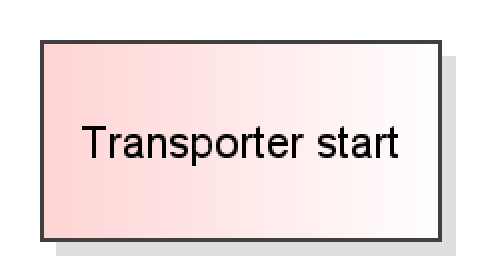
\includegraphics[width=2cm]{imageModelElementTransportTransporterSource.png}
\vspace{-22pt}
\end{wrapfigure}

A transporter start element allows to transport a client to any
transport destination (see page \pageref{ref:ModelElementTransportDestination}) 
element. How much time is needed for the transport and to which
transport destination element the client is transported can be set up
in the transporter start element. 
There is no need for a connection edge between the transport origin element
and the transport destination element for routing clients from the origin to the
destination.
In comparison to the  transport origin (see page \pageref{ref:ModelElementTransportSource}) 
element at a transporter start element no resources (which do not have a physical location)
are used but transporters which move between the stations.

\subsection*{Settings}

The name of the transporter start element has no further meaning.

On the dialog page \textbf{Transporter}, it is possible to specify which type
of transporter is to be used to pick up for waiting clients, how many clients
have to wait before a transporter is being requested, and what priority the
transporter start element should have when requesting transporters.
Furthermore, even without waiting clients, transporters can be requested,
which then park in the element. Again, a priority and maximum capacity can be specified.

On the dialog page \textbf{Routing destinations} target stations for transfering the
clients can be registered. Conditions or client types can be specified for the transport
destinations. Alternatively the clients sequence or a clients text property can be used to determine
the transport destination.

On the dialog page \textbf{Priorities} a priority for waiting clients
to get a place in an arriving transporter can be defined.
The variable "w" indicates here the client's previous waiting time at the current station.
(In all other cases "w" is the total waiting time of the current client.)

On the dialog page \textbf{Leave section} optionally an enter section station can be specified.
When the transport of the client starts, the corresponding section will be left.


\section{Transporter way point}
\label{ref:ModelElementWayPoint}

\begin{wrapfigure}{l}{2.5cm}
\vspace{-22pt}

\includegraphics[width=2cm]{imageModelElementWayPoint.png}
\vspace{-22pt}
\end{wrapfigure}

Way points are visited by transporters during the animation on their way from an 
origin to a destination station. They have no meaning for the simulation itself.

\subsection*{Settings}

For each way point can be set on which routes from which origin to which
destination station they are to be visited.

\textbf{Node:}~\\
Creating paths by editing the way point settings directly is very expensive.
To simplify this process the paths editor 
which can be accessed via the context menu of a way point can be used.





\chapter{Data input/output}

\section{Input}
\label{ref:ModelElementInput}

\begin{wrapfigure}{l}{2.5cm}
\vspace{-22pt}
\includegraphics[width=2cm]{imageModelElementInput.png}
\vspace{-22pt}
\end{wrapfigure}

If a client passes through this element, a numerical value is read from a file
and assigned to a variable. The reading position then is moved by one line.
If a client is reaching the end of the file, different actions can be processed.

\subsection*{Settings}

The name of the input element has no further meaning for the simulation.
You need to set up the name of the input file to be read, the intended behavior
at the end of the file and the name of the variable where the value is to
be assigned to.

By using the pseudo variables "w", "t" and "p" you can access the waiting time, the transfer time and the
process time of the current client (each on second base) for reading and for writing. Additionally you can
write to a client object data field by using "ClientData(index)" as target variable or a text to a client-based
key by using "ClientData('key')".

\subsection*{Alternative}

The Input (JS) element (see page \pageref{ref:ModelElementInputJS}) allows to define more complex processings
of the input values. On the other side the Javascript programs to be executed with the input values
will need much more computing time to be executed during simulation.


\section{Input (DB)}
\label{ref:ModelElementInputDB}

\begin{wrapfigure}{l}{2.5cm}
\vspace{-22pt}
\includegraphics[width=2cm]{imageModelElementInputDB.png}
\vspace{-22pt}
\end{wrapfigure}

If a client passes through this element, a numerical value is read from a
database table and assigned to a variable. The reading position then is moved by one line.
If a client is reaching the end of the file, different actions can be processed.

\subsection*{Settings}

The name of the input element has no further meaning for the simulation.
Next to the database connection settings, the table and the column to load
the intended behavior at the end of the file and the name of the variable
where the value is to be assigned to have to be specified.

By using the pseudo variables "w", "t" and "p" you can access the waiting time, the transfer time and the
process time of the current client (each on second base) for reading and for writing. Additionally you can
write to a client object data field by using "ClientData(index)" as target variable or a text to a client-based
key by using "ClientData('key')".


\section{Input (DDE)}
\label{ref:ModelElementInputDDE}

\begin{wrapfigure}{l}{2.5cm}
\vspace{-22pt}
\includegraphics[width=2cm]{imageModelElementInputDDE.png}
\vspace{-22pt}
\end{wrapfigure}

If a client passes through this element, a numerical value is read via DDE from an
Excel table and assigned to a variable. The reading position then is moved by one line.
If a client is reaching the end of the file, different actions can be processed.

\subsection*{Settings}

The name of the input element has no further meaning for the simulation.
Next to the DDE connection settings the intended behavior at the end of the file and the name of the variable
where the value is to be assigned to have to be specified.

By using the pseudo variables "w", "t" and "p" you can access the waiting time, the transfer time and the
process time of the current client (each on second base) for reading and for writing. Additionally you can
write to a client object data field by using "ClientData(index)" as target variable or a text to a client-based
key by using "ClientData('key')".


\section{Input (Script)}
\label{ref:ModelElementInputJS}

\begin{wrapfigure}{l}{2.5cm}
\vspace{-22pt}
\includegraphics[width=2cm]{imageModelElementInputJS.png}
\vspace{-22pt}
\end{wrapfigure}

If a client passes through this element, a numerical value is read from a file
and make available in an user-defined Javascript or Java program.

\subsection*{Settings}

The name of the input element has no further meaning for the simulation.
You need to set up the name of the input file to be read, the intended behavior
at the end of the file and the script to be executed.
The script commands to be executed are defined in \textbf{Javascript} or in \textbf{Java}.
Next to the default Javascript or Java commands some 
additional Javascript commands or
additional Java commands 
are available for accessing the simulation data.

\subsection*{Alternative}

The script based variable assignment allows maximum flexibility, but takes a comparatively long
computing time. A faster option for assigning variables is using the
Input element (see page \pageref{ref:ModelElementInput}) .


\section{Output}
\label{ref:ModelElementOutput}

\begin{wrapfigure}{l}{2.5cm}
\vspace{-22pt}
\includegraphics[width=2cm]{imageModelElementOutput.png}
\vspace{-22pt}
\end{wrapfigure}

If a client passes through this element, some definable status information are written to an output file.

\subsection*{Settings}

The name of the output element has no further meaning. The name of the file to which the data is to be written
can be specified using the filename field. Multiple data can be written for each client event whose order and
values can be defined via the table rows in the setting dialog of the output element.

\subsection*{Alternative}

The Output (JS) element (see page \pageref{ref:ModelElementOutputJS}) allows to define more complex output formats
for the simulation data. On the other side the Output (JS) element will need much more computing time to be
executed during simulation.


\section{Output (DB)}
\label{ref:ModelElementOutputDB}

\begin{wrapfigure}{l}{2.5cm}
\vspace{-22pt}
\includegraphics[width=2cm]{imageModelElementOutputDB.png}
\vspace{-22pt}
\end{wrapfigure}

If a client passes through this element, some definable status information are written to a database table.

\subsection*{Settings}

The name of the Output (DB) element has no further meaning. One has to specify settings to connect to
the database and the name of a table in the database into which the information are to be written.  
Multiple data can be written in different table columns for each client event. Each client arrival
adds a new row the database table.


\section{Output (DDE)}
\label{ref:ModelElementOutputDDE}

\begin{wrapfigure}{l}{2.5cm}
\vspace{-22pt}
\includegraphics[width=2cm]{imageModelElementOutputDDE.png}
\vspace{-22pt}
\end{wrapfigure}

If a client passes through this element, some definable status information are written via DDE to an Excel table.

\subsection*{Settings}

The name of the Output (DDE) element has no further meaning. One has to specify the DDE connect settings.  
Multiple data can be written in different table columns for each client event. Each client arrival
adds a new row the table.


\section{Output (Log)}
\label{ref:ModelElementOutputLog}

\begin{wrapfigure}{l}{2.5cm}
\vspace{-22pt}
\includegraphics[width=2cm]{imageModelElementOutputLog.png}
\vspace{-22pt}
\end{wrapfigure}

If a client passes through this element, some definable status information are written to the log output.
If loggig is not activated, no output will happen.

\subsection*{Settings}

The name of the output element has no further meaning. Multiple data can be written for each client event whose order and
values can be defined via the table rows in the setting dialog of the output element.


\section{Output (Script)}
\label{ref:ModelElementOutputJS}

\begin{wrapfigure}{l}{2.5cm}
\vspace{-22pt}
\includegraphics[width=2cm]{imageModelElementOutputJS.png}
\vspace{-22pt}
\end{wrapfigure}

If a client passes through this element, some status information definable via
a Javascript or a Jaava program are written to an output file.

\subsection*{Settings}

The name of the output element has no further meaning. The name of the file to which the data is to be written
can be specified using the filename field. The script commands to be executed are defined in \textbf{Javascript}
or in \textbf{Java}. Next to the default Javascript and Java commands some
additional Javascript commands or additional Java commands 
are available for accessing the simulation data.

\subsection*{Alternative}

The definition of script defined output allows maximum flexibility, but takes a comparatively long
computing time. A faster option for writing out simulation data is to use the
Output element (see page \pageref{ref:ModelElementOutput}) .


\section{Recording}
\label{ref:ModelElementRecord}

\begin{wrapfigure}{l}{2.5cm}
\vspace{-22pt}
\includegraphics[width=2cm]{imageModelElementRecord.png}
\vspace{-22pt}
\end{wrapfigure}

If a client passes through this element, the values of one or two user-defined expressions
are recorded to the statistics. If one expression is given, the values will be presented
as a line diagrame. On two expressions a X-Y points diagram will be created.

\subsection*{Limitations}

In contrast to an Output element (see page \pageref{ref:ModelElementOutput}) the data recoding element
is no recording to an external file but will keep the recorded values in memory to be able to
directly present them in the statistics viewer. For this reason the maximum number of recorded
values is limited to 2 million. When storing the statistics to a xml file and when displaying
line diagrams, up to 2 million values are used. For X-Y point diagrams and in tables only up to
2$^{17}$ values will be used.

\subsection*{Settings}

The data will be recorded in the statistics under the name of the data recording element. 
At least one expression whose values are to be recorded has to be specified.
The second expression is optional.





\chapter{Flow control logic}

\section{Do}
\label{ref:ModelElementLogicDo}

\begin{wrapfigure}{l}{2.5cm}
\vspace{-22pt}
\includegraphics[width=2cm]{imageModelElementLogicDo.png}
\vspace{-22pt}
\end{wrapfigure}

The Do element always forwards clients to the next station.
It is used as the starting point of loops and as jump target
for Until (see page \pageref{ref:ModelElementLogicUntil}) stations.

\subsection*{Settings}

The name of the station has no meaning for the simulation.


\section{Else}
\label{ref:ModelElementLogicElse}

\begin{wrapfigure}{l}{2.5cm}
\vspace{-22pt}
\includegraphics[width=2cm]{imageModelElementLogicElse.png}
\vspace{-22pt}
\end{wrapfigure}

The Else element forwards the clients either to the directly following station or to the
next EndIf (see page \pageref{ref:ModelElementLogicEndIf}) station depending if the condition
on the previous If (see page \pageref{ref:ModelElementLogicIf}) or
ElseIf element (see page \pageref{ref:ModelElementLogicElseIf}) was fulfilled or not.
This allows to implement a graphical flow control similar to classical programming
languages.

\subsection*{Settings}

The name of the station has no meaning for the simulation.


\section{ElseIf}
\label{ref:ModelElementLogicElseIf}

\begin{wrapfigure}{l}{2.5cm}
\vspace{-22pt}
\includegraphics[width=2cm]{imageModelElementLogicElseIf.png}
\vspace{-22pt}
\end{wrapfigure}

The ElseIf elements forwards the clients either to the directly following station or to the
next ElseIf (see page \pageref{ref:ModelElementLogicElseIf}) ,
Else (see page \pageref{ref:ModelElementLogicElse}) or
EndIf (see page \pageref{ref:ModelElementLogicEndIf}) station depending if the condition
on the previous If (see page \pageref{ref:ModelElementLogicIf}) or
ElseIf element (see page \pageref{ref:ModelElementLogicElseIf}) was fulfilled and if the
condition on this station is fulfilled.
This allows to implement a graphical flow control similar to classical programming
languages.	

\subsection*{Settings}

The name of the station has no meaning for the simulation.
The next station for forwarding the clients to is selected by the given condition.


\section{EndIf}
\label{ref:ModelElementLogicEndIf}

\begin{wrapfigure}{l}{2.5cm}
\vspace{-22pt}
\includegraphics[width=2cm]{imageModelElementLogicEndIf.png}
\vspace{-22pt}
\end{wrapfigure}

The EndIf element ends a flow control chain
started with an
If element (see page \pageref{ref:ModelElementLogicEndIf}) .

\subsection*{Settings}

The name of the station has no meaning for the simulation.


\section{EndWhile}
\label{ref:ModelElementLogicEndWhile}

\begin{wrapfigure}{l}{2.5cm}
\vspace{-22pt}
\includegraphics[width=2cm]{imageModelElementLogicEndWhile.png}
\vspace{-22pt}
\end{wrapfigure}

The EndWhile element ends a loop started by a
While element (see page \pageref{ref:ModelElementLogicWhile}) .
The client will be routed to the While element.
The While element checks if the condition is still
fulfilled. If not, the client will be routed to the
element following the EndWhile element. Otherwise
the loop will be executed another time.

\subsection*{Settings}

The name of the station has no meaning for the simulation.


\section{If}
\label{ref:ModelElementLogicIf}

\begin{wrapfigure}{l}{2.5cm}
\vspace{-22pt}
\includegraphics[width=2cm]{imageModelElementLogicIf.png}
\vspace{-22pt}
\end{wrapfigure}

The If element forwards clients depending on a condition either to the directly following station
(if the condition is fulfilled) or to the next ElseIf (see page \pageref{ref:ModelElementLogicElseIf}) ,
Else (see page \pageref{ref:ModelElementLogicElse}) or EndIf (see page \pageref{ref:ModelElementLogicEndIf}) 
station. This allows to implement a graphical flow control similar to classical programming
languages.

\subsection*{Settings}

The name of the station has no meaning for the simulation.
The next station for forwarding the clients to is selected by the given condition.


\section{Until}
\label{ref:ModelElementLogicUntil}

\begin{wrapfigure}{l}{2.5cm}
\vspace{-22pt}
\includegraphics[width=2cm]{imageModelElementLogicUntil.png}
\vspace{-22pt}
\end{wrapfigure}

The Until element ends a loop started by a
Do element (see page \pageref{ref:ModelElementLogicDo}) .
The client will be forwarded to the Do element again,
as long as the condition is not yet fulfilled.

\subsection*{Settings}

The name of the station has no meaning for the simulation.
The next station for forwarding the clients to is selected by the given condition.


\section{While}
\label{ref:ModelElementLogicWhile}

\begin{wrapfigure}{l}{2.5cm}
\vspace{-22pt}
\includegraphics[width=2cm]{imageModelElementLogicWhile.png}
\vspace{-22pt}
\end{wrapfigure}

The While element forwards clients depending on a condition either to the directly following station
(if the condition is fulfilled) or to the next EndWhile (see page \pageref{ref:ModelElementLogicEndWhile}) 
station. This allows to implement a graphical flow control similar to classical programming
languages.

\subsection*{Settings}

The name of the station has no meaning for the simulation.
The next station for forwarding the clients to is selected by the given condition.





\chapter{Analog values}

\section{Analog value}
\label{ref:ModelElementAnalogValue}

\begin{wrapfigure}{l}{2.5cm}
\vspace{-22pt}
\includegraphics[width=2cm]{imageModelElementAnalogValue.png}
\vspace{-22pt}
\end{wrapfigure}

The element contains a value which changes by a rate over the time.
The value and the rate can be changed during run time by a
Change analog value element (see page \pageref{ref:ModelElementAnalogAssign}) .

If a minimum and a maximum value for the analog value are defined,
the \textbf{fill level} is drawn in the element shape.

\subsection*{Settings}

The name of the analog value element has no further meaning for the simulation.
Next to the initial value, the initial change rate and an optional minimum and maximum value
one can specify how often the discreet simulation should be informed about the change of
the continuous value.


\section{Change analog value}
\label{ref:ModelElementAnalogAssign}

\begin{wrapfigure}{l}{2.5cm}
\vspace{-22pt}
\includegraphics[width=2cm]{imageModelElementAnalogAssign.png}
\vspace{-22pt}
\end{wrapfigure}

If a client passes this element, in one or more
Analog value (see page \pageref{ref:ModelElementAnalogValue}) and
Tank elements (see page \pageref{ref:ModelElementTank}) 
new values and change rates will be set up.

\subsection*{Settings}

The name of the analog value element has no further meaning for the simulation.
In the element can be set up which values and rates will be changed in which element.


\section{Flow}
\label{ref:ModelElementTankFlowByClient}

\begin{wrapfigure}{l}{2.5cm}
\vspace{-22pt}
\includegraphics[width=2cm]{imageModelElementTankFlowByClient.png}
\vspace{-22pt}
\end{wrapfigure}

A flow is a connection between two Tanks (see page \pageref{ref:ModelElementTank}) 
(or to be more precise between two valves at two different tanks).
Or between the flow source and a tank or between a tank and a flow destination.

A flow defines how many unit are to be transported from the source to the target
or how long the flow is to be active.

The flow will be activated by a client passing through the element.

\subsection*{Settings}

The name of the flow element has no further meaning for the simulation.
For each flow, a source and a destination have to be specified.
It is also necessary to define how long the flow should be active.
The duration of activity can be defined as a time span, a flow quantity or by a stop signal.


\section{Flow (signal)}
\label{ref:ModelElementTankFlowBySignal}

\begin{wrapfigure}{l}{2.5cm}
\vspace{-22pt}
\includegraphics[width=2cm]{imageModelElementTankFlowBySignal.png}
\vspace{-22pt}
\end{wrapfigure}

A flow is a connection between two Tanks (see page \pageref{ref:ModelElementTank}) 
(or to be more precise between two valves at two different tanks).
Or between the flow source and a tank or between a tank and a flow destination.

A flow defines how many unit are to be transported from the source to the target
or how long the flow is to be active.

The flow will be activated by a signal.

\subsection*{Settings}

The name of the flow element has no further meaning for the simulation.
For each flow, a starting signal has to be specified.
Additionally a source and a destination have to be specified for each flow
and it is also necessary to define how long the flow should be active.
The duration of activity can be defined as a time span, a flow quantity or by a stop signal.


\section{Sensor}
\label{ref:ModelElementTankSensor}

\begin{wrapfigure}{l}{2.5cm}
\vspace{-22pt}
\includegraphics[width=2cm]{imageModelElementTankSensor.png}
\vspace{-22pt}
\end{wrapfigure}

A sensor element triggers a signal just like a Signal element (see page \pageref{ref:ModelElementSignal}) .
But in constrast to the signal element the signal ist not triggered on a client arrival
but when a threshold value at a connected Tank element (see page \pageref{ref:ModelElementTank}) 
is exceeded or underflowed.

\subsection*{Settings}

The name of the sensor element is also the name of the signal that is triggered when the condition is matched.
As condition, either the exceeding or falling below a certain threshold value in a tank can be used.


\section{Tank}
\label{ref:ModelElementTank}

\begin{wrapfigure}{l}{2.5cm}
\vspace{-22pt}
\includegraphics[width=2cm]{imageModelElementTank.png}
\vspace{-22pt}
\end{wrapfigure}

The element contains a value which can change over the time.
Each tank contains one or more valves. Flows (see Flow (see page \pageref{ref:ModelElementTankFlowByClient}) 
and Flow (Signal) elements (see page \pageref{ref:ModelElementTankFlowBySignal}) )
can be connected to the valves.The valves define how much of the content of the tank
can flow per time unit, the flows define how much is to be transported or how long
the flow should be active.

In contrast to the Analog value elements (see page \pageref{ref:ModelElementAnalogValue}) 
the value of a tank can never be negative and always has an upper limit (the capacity of the tank).

It is not necessary to connect a flow to a valve at all times.
If a flow is connect to a valve, it will be served directly.
If several flows are connect, only one flow will be served at any one time.
Only when the first time flow has been processed, the next is activated.
This means multiple flows will not share the available flow rate of a valve.

\subsection*{Settings}

The name of the tank element has no further meaning for the simulation.
Next to the capacity, the initial value and the valves with their maximum flow per time unit
one can specify how often the discreet simulation should be informed about the change of
the continuous value.


\section{Valve setup}
\label{ref:ModelElementTankValveSetup}

\begin{wrapfigure}{l}{2.5cm}
\vspace{-22pt}
\includegraphics[width=2cm]{imageModelElementTankValveSetup.png}
\vspace{-22pt}
\end{wrapfigure}

If a client passes through this element, the maximum flow of one or more valves
at some Tank elements (see page \pageref{ref:ModelElementTank}) is changed.

\subsection*{Settings}

The name of the valve setup element has no further meaning for the simulation.
One can specify any number of valves which are to be set to a new maximum flow.





\chapter{Animation}

\section{Analogue scale display}
\label{ref:ModelElementAnimationPointerMeasuring}

\begin{wrapfigure}{l}{2.5cm}
\vspace{-22pt}
\includegraphics[width=2cm]{imageModelElementAnimationPointerMeasuring.png}
\vspace{-22pt}
\end{wrapfigure}

An analogue scale display element makes it possible to display the current
value of an expression on an analogue measuring scale by positioning the pointer.

\subsection*{Settings}

The name of the simulation time element has no further meaning.
In addition to the calculation expression to be evaluated,
the maximum value of the scale must be specified.


\section{Animation image}
\label{ref:ModelElementAnimationImage}

\begin{wrapfigure}{l}{2.5cm}
\vspace{-22pt}
\includegraphics[width=2cm]{imageModelElementAnimationImage.png}
\vspace{-22pt}
\end{wrapfigure}

In the animation image element, several images can be specified
which are displayed during the animation of the model
depending on certain conditions.

\subsection*{Settings}

The name of the animation image element has no further meaning.
You can define a condition for each picture. The list of images and conditions
is always processed from top to bottom during the animation.
The image corresponding to the first fulfilled condition is displayed.
If none of the specified conditions is true, the last image in the list
(to which no condition can be specified) will be displayed.


\section{Icon: Person - blue}
\label{ref:ModelElementClientIcon}

\begin{wrapfigure}{l}{2.5cm}
\vspace{-22pt}
\includegraphics[width=2cm]{imageModelElementClientIcon.png}
\vspace{-22pt}
\end{wrapfigure}

The icon element assigns a new animation icon to the clients who pass this element.

\subsection*{Settings}

The name of the icon element has no further meaning. The icon, which is to be assigned to the
clients who pass this element, can be selected via the icon selection field.


\section{LCD display}
\label{ref:ModelElementAnimationLCD}

\begin{wrapfigure}{l}{2.5cm}
\vspace{-22pt}
\includegraphics[width=2cm]{imageModelElementAnimationLCD.png}
\vspace{-22pt}
\end{wrapfigure}

An LCD display element allows to display the current value of an expression
in the form of a 7 segment display with an adjustable number of digits.
Only the integer part of the value is output. 

\subsection*{Settings}

The name of the LCD display element has no further meaning.
In addition to the expression to be evaluated, the number of
7 segment digits to be displayed and the color of the active
segments can be set.


\section{Script result as text}
\label{ref:ModelElementAnimationTextJS}

\begin{wrapfigure}{l}{2.5cm}
\vspace{-22pt}
\includegraphics[width=2cm]{imageModelElementAnimationTextJS.png}
\vspace{-22pt}
\end{wrapfigure}

The simulation data as a text element allows to display data in text form during the animation of a model.
The results of a script will be displayed.

\subsection*{Settings}

The script code can contain any Javascript or Java commands as well as some
special Javascript commands or special Java commands 
for accessing the simulation system.


\section{Show recorded data}
\label{ref:ModelElementAnimationRecord}

\begin{wrapfigure}{l}{2.5cm}
\vspace{-22pt}
\includegraphics[width=2cm]{imageModelElementAnimationRecord.png}
\vspace{-22pt}
\end{wrapfigure}

Stations of the type "Show recorded data" allow to display the values
recorded at a Data recording (see page \pageref{ref:ModelElementRecord}) station
during animation. The diagram type (line diagram or X-Y points diagram) is
chosen automatically from the type of the data recording station (one or two values).

\subsection*{Settings}

The name of the data recording display element has no further meaning. For
displaying data a corresponding data recording element has to be chosen.
Additional the number of data points to be displayed can be configured.
(The most recent data will be displayed.)


\section{Simulation data as bar plot}
\label{ref:ModelElementAnimationBar}

\begin{wrapfigure}{l}{2.5cm}
\vspace{-22pt}
\includegraphics[width=2cm]{imageModelElementAnimationBar.png}
\vspace{-22pt}
\end{wrapfigure}

The simulation data as a bar element allows to display the value of an expression in the form of a dynamically sized
bar during the animation of a model. Each computable expression can be displayed (which includes the functions for
determining queue lengths at individual stations as well as access to all user-defined simulation variables).
For classical simulation, the simulation data elements are without further meaning.

\subsection*{Settings}

The name of the simulation data element has no further meaning.
For the expression to be displayed, a range can be set which the bar should represent.


\section{Simulation data as stacked bar plot}
\label{ref:ModelElementAnimationBarStack}

\begin{wrapfigure}{l}{2.5cm}
\vspace{-22pt}
\includegraphics[width=2cm]{imageModelElementAnimationBarStack.png}
\vspace{-22pt}
\end{wrapfigure}

The simulation data as a stacked bar element allows to display the values of multiple expressions in the form of
a dynamically sized bar consisting of multiple segments during the animation of a model. Each computable expression
can be displayed (which includes the functions for determining queue lengths at individual stations as well as access
to all user-defined simulation variables). For classical simulation, the simulation data elements are without further meaning.

\subsection*{Settings}

The name of the simulation data element has no further meaning.
For the sum of the expressions to be displayed, a maximum value can be set 
otherwise the segments are scaled to fill the entry bar area.


\section{Simulation data as text}
\label{ref:ModelElementAnimationText}

\begin{wrapfigure}{l}{2.5cm}
\vspace{-22pt}
\includegraphics[width=2cm]{imageModelElementAnimationText.png}
\vspace{-22pt}
\end{wrapfigure}

The simulation data as a text element allows to display data in text form during the animation of a model.
Any computable expression can be displayed (which includes the functions for determining queue lengths at
individual stations as well as access to all user-defined simulation variables). The output is in text form
on the drawing surface. For classical simulation, the simulation data elements are without further meaning.

\subsection*{Settings}

The name of the simulation data element is displayed on the drawing area directly above the value.
You can select whether the element should display the current simulation time or any computable expression.
If an expression is displayed, the numerical value can also optionally be displayed as a percentage
(i.e., 70% instead of 0.7).


\section{Simulation data bar chart}
\label{ref:ModelElementAnimationBarChart}

\begin{wrapfigure}{l}{2.5cm}
\vspace{-22pt}
\includegraphics[width=2cm]{imageModelElementAnimationBarChart.png}
\vspace{-22pt}
\end{wrapfigure}

A simulation data bar chart allows you to display the value of one or more expressions
in the form of a bar chart during the animation of a model.
All computable expressions can be displayed (which includes the functions for determining queue
lengths at individual stations as well as access to all user-defined simulation variables).
For classical simulation, the simulation data elements are without further meaning.

\subsection*{Settings}

The name of the simulation data bar chart element has no further meaning.
For the expressions to be displayed in the bar chart, any valid expressions can be used;
additional a value range can be set.


\section{Simulation data line chart}
\label{ref:ModelElementAnimationDiagram}

\begin{wrapfigure}{l}{2.5cm}
\vspace{-22pt}
\includegraphics[width=2cm]{imageModelElementAnimationDiagram.png}
\vspace{-22pt}
\end{wrapfigure}

A simulation data line chart allows you to continuously display the value of one or more expressions
in the form of a continuously updated line graph during the animation of a model.
All computable expressions can be displayed (which includes the functions for determining queue
lengths at individual stations as well as access to all user-defined simulation variables).
For classical simulation, the simulation data elements are without further meaning.

\subsection*{Settings}

The name of the simulation data line chart element has no further meaning.
For the expressions to be displayed in the line chart, any valid expressions can be used;
a value range can be set for each expression.


\section{Simulation data pie chart}
\label{ref:ModelElementAnimationPieChart}

\begin{wrapfigure}{l}{2.5cm}
\vspace{-22pt}
\includegraphics[width=2cm]{imageModelElementAnimationPieChart.png}
\vspace{-22pt}
\end{wrapfigure}

A simulation data pie chart allows you to continuously display the relationship
of several values to each other as a pie chart during the animation of a model.
For classical simulation, the simulation data elements are without further meaning.

\subsection*{Settings}

The name of the simulation data pie chart element has no further meaning.
For the expressions to be displayed in the bar chart, any valid expressions can be used.


\section{Simulation data traffic lights}
\label{ref:ModelElementAnimationTrafficLights}

\begin{wrapfigure}{l}{2.5cm}
\vspace{-22pt}
\includegraphics[width=2cm]{imageModelElementAnimationTrafficLights.png}
\vspace{-22pt}
\end{wrapfigure}

The simulation data traffic lights element allows to display the value of an expression during the animation
in the form of a traffic light, which distinguishes two or three states. Each computable expression can be
displayed (which includes the functions for determining queue lengths at individual stations as well as
access to all user-defined simulation variables). For classical simulation, the simulation data elements
are without further meaning.

\subsection*{Settings}

The name of the simulation data traffic lights element has no further meaning.
In the case of a traffic light with three lights, the evaluation is carried out from the top to the bottom:
The condition for the yellow light is only checked if the condition for the red light is not already fulfilled.


\section{Simulation time}
\label{ref:ModelElementAnimationClock}

\begin{wrapfigure}{l}{2.5cm}
\vspace{-22pt}
\includegraphics[width=2cm]{imageModelElementAnimationClock.png}
\vspace{-22pt}
\end{wrapfigure}

The simulation time element allows to display the current simulation time
(or any other seconds-based value) in form of an analogue clock during animation.
For classical simulation, the simulation data elements are without further meaning.

\subsection*{Settings}

The name of the simulation time element has no further meaning.
For the expression to be displayed in the clock any expression the simulation can calculate can be used.


\section{Text by simulation data}
\label{ref:ModelElementAnimationTextSelect}

\begin{wrapfigure}{l}{2.5cm}
\vspace{-22pt}
\includegraphics[width=2cm]{imageModelElementAnimationTextSelect.png}
\vspace{-22pt}
\end{wrapfigure}

The text by simulation data element allows to display different strings depending on some conditions.
Any computable expression can be used as a condition to select as string (which includes the functions for
determining queue lengths at individual stations as well as access to all user-defined simulation
variables). The output is in text form on the drawing surface. For classical simulation, the simulation
data elements are without further meaning.

\subsection*{Settings}

The name of the simulation data element is displayed on the drawing area directly above the conditional string.
You can define any number of conditions and strings and also one default string which is displayed,
if non of the conditions apply.





\chapter{Animation - Interactive}

\section{Button}
\label{ref:ModelElementInteractiveButton}

\begin{wrapfigure}{l}{2.5cm}
\vspace{-22pt}
\includegraphics[width=2cm]{imageModelElementInteractiveButton.png}
\vspace{-22pt}
\end{wrapfigure}

"Button" elements are not connected to the regular flow of clients.
They can only be used during animation and will trigger one or more
action when they are clicked.

These action types can be triggered by an "Button" element:

\begin{itemize}
  \item Assigning a value to a variable 
  \item Changing the value at an element containing an analog value
  (Analog value (see page \pageref{ref:ModelElementAnalogValue}) or Tank (see page \pageref{ref:ModelElementTank}) )
  \item Triggering a signal 
  \item Running some Javascript or Java code 
\end{itemize}

\subsection*{Settings}

The name of the "Button" element has no further meaning for the simulation.
In each "Button" element any number of actions can be defined. The actions will
be executed if the button is clicked during animation.


\section{Checkbox}
\label{ref:ModelElementInteractiveCheckbox}

\begin{wrapfigure}{l}{2.5cm}
\vspace{-22pt}
\includegraphics[width=2cm]{imageModelElementInteractiveCheckbox.png}
\vspace{-22pt}
\end{wrapfigure}

"Checkbox" elements are not connected to the regular flow of clients.
They can only be used during animation for adjusting the value of
variables.

\subsection*{Settings}

The name of the "Checkbox" element has no further meaning for the simulation.
In each "Checkbox" element the name of the variable to which values are to
be assigned has to be specified. Additionally the value which should be
applied when activating and unactivating the checkbox during the animation
have to be specified.  


\section{Radiobutton}
\label{ref:ModelElementInteractiveRadiobutton}

\begin{wrapfigure}{l}{2.5cm}
\vspace{-22pt}
\includegraphics[width=2cm]{imageModelElementInteractiveRadiobutton.png}
\vspace{-22pt}
\end{wrapfigure}

"Radiobutton" elements are not connected to the regular flow of clients.
They can only be used during animation for adjusting the value of
variables.

\subsection*{Settings}

The name of the "Radiobutton" element has no further meaning for the simulation.
In each "Radiobutton" element the name of the variable to which values are to
be assigned has to be specified. Additionally the value which should be
applied when clicking the radiobutton during the animation has to be specified.  


\section{Slider}
\label{ref:ModelElementInteractiveSlider}

\begin{wrapfigure}{l}{2.5cm}
\vspace{-22pt}
\includegraphics[width=2cm]{imageModelElementInteractiveSlider.png}
\vspace{-22pt}
\end{wrapfigure}

"Slider" elements are not connected to the regular flow of clients.
They can only be used during animation for adjusting the value of
variables.

\subsection*{Settings}

The name of the "Slider" element has no further meaning for the simulation.
In each "Slider" element has to specify the name of the variable and the
range in which its to be changed when the element is clicked during the
animation.





\chapter{Optical decorations}

\section{Connection vertex}
\label{ref:ModelElementVertex}

\begin{wrapfigure}{l}{2.5cm}
\vspace{-22pt}
\includegraphics[width=2cm]{imageModelElementVertex.png}
\vspace{-22pt}
\end{wrapfigure}

Connection edges always run in a straight line from the output component
to the target component. In order to be able to present the sequences more clearly, connection vertices can be used.
One or more edges can run into a connecting vertex, and one edge can - if necessary in a different direction - run out
of the connecting vertex. In this way, paths can be optically deflected.

\subsection*{Settings}

Connection vertices have no properties. Also, a connection vertex can not get a name.


\section{Description text}
\label{ref:ModelElementText}

\begin{wrapfigure}{l}{2.5cm}
\vspace{-22pt}
\includegraphics[width=2cm]{imageModelElementText.png}
\vspace{-22pt}
\end{wrapfigure}

Description texts have no function for the course of the simulation
and serve only for the optical design of the model
(for example, for labeling partial components, transitions, etc.).

\subsection*{Settings}

In addition to the text itself, a font family and a font size can also be set for each description text element.


\section{Ellipse}
\label{ref:ModelElementEllipse}

\begin{wrapfigure}{l}{2.5cm}
\vspace{-22pt}
\includegraphics[width=2cm]{imageModelElementEllipse.png}
\vspace{-22pt}
\end{wrapfigure}

The line (see page \pageref{ref:ModelElementLine}) , the rectangle (see page \pageref{ref:ModelElementRectangle}) 
and the ellipse element are only used for the optical design of the model and have no significance for the simulation.

\subsection*{Settings}

The name of the ellipse element has no further meaning.


\section{Image}
\label{ref:ModelElementImage}

\begin{wrapfigure}{l}{2.5cm}
\vspace{-22pt}
\includegraphics[width=2cm]{imageModelElementImage.png}
\vspace{-22pt}
\end{wrapfigure}

Images are only for the optical design of the model and have no significance for the simulation.

\subsubsection*{Note:}

Images can also be dragged directly to the canvas by drag\&drop.

\subsection*{Settings}

The name of the image element has no further meaning.


\section{Line}
\label{ref:ModelElementLine}

\begin{wrapfigure}{l}{2.5cm}
\vspace{-22pt}
\includegraphics[width=2cm]{imageModelElementLine.png}
\vspace{-22pt}
\end{wrapfigure}

The line, the rectangle (see page \pageref{ref:ModelElementRectangle}) and the
ellipse element (see page \pageref{ref:ModelElementEllipse}) 
are only used for the optical design of the model and have no significance for the simulation.

\subsection*{Settings}

The name of the line element has no further meaning.


\section{note}
\label{ref:ModelElementNote}

\begin{wrapfigure}{l}{2.5cm}
\vspace{-22pt}
\includegraphics[width=2cm]{imageModelElementNote.png}
\vspace{-22pt}
\end{wrapfigure}

Notes have no meaning for simulation or animation.
Notes are only used for the user to record important comments about the model.

An overview of all notes available in the model can be accessed via
the Notes menu item in the model menu.

\subsection*{Settings}

In addition to the text itself, the icon which is used for displaying
the note on the drawing surface can be selected.


\section{Rectangle}
\label{ref:ModelElementRectangle}

\begin{wrapfigure}{l}{2.5cm}
\vspace{-22pt}
\includegraphics[width=2cm]{imageModelElementRectangle.png}
\vspace{-22pt}
\end{wrapfigure}

The line (see page \pageref{ref:ModelElementLine}) -, the ellipse (see page \pageref{ref:ModelElementEllipse}) and
das rectangle Element are only used for the optical design of the model and have no significance for the simulation.

\subsection*{Einstellungen}

The name of the rectangle element has no further meaning.





\chapter{Others}

\section{Action}
\label{ref:ModelElementAction}

\begin{wrapfigure}{l}{2.5cm}
\vspace{-22pt}
\includegraphics[width=2cm]{imageModelElementAction.png}
\vspace{-22pt}
\end{wrapfigure}

"Action" elements are not connected to the regular flow of clients.
"Action" elements trigger different actions when some conditions are matched.

These action types can be triggered by an "Action" element:

\begin{itemize}
  \item Assigning a value to a variable 
  \item Changing the value at an element containing an analog value
  (Analog value (see page \pageref{ref:ModelElementAnalogValue}) or Tank (see page \pageref{ref:ModelElementTank}) )
  \item Triggering a signal 
  \item Running some Javascript or Java code 
\end{itemize}

\subsection*{Settings}

The name of the "Action" element has no further meaning for the simulation.
In each "Action" element any number of actions can be defined. Each action
consists of a trigger (a condition to be fulfilled, an exceeded threshold value or a signal)
and some action to be executed (see above).


\section{Reference}
\label{ref:ModelElementReference}

\begin{wrapfigure}{l}{2.5cm}
\vspace{-22pt}
\includegraphics[width=2cm]{imageModelElementReference.png}
\vspace{-22pt}
\end{wrapfigure}

The reference element allows to use the settings from some other element.
If a client passes the reference element the processing which would happen
if the client would have passed the element to which is referenced is done.

\subsection*{Settings}

The name of the reference element has no further meaning for the simulation.
An element from which the settings are to be used has to be specified.


\section{Statistics}
\label{ref:ModelElementUserStatistic}

\begin{wrapfigure}{l}{2.5cm}
\vspace{-22pt}
\includegraphics[width=2cm]{imageModelElementUserStatistic.png}
\vspace{-22pt}
\end{wrapfigure}

If a client passes through this element, some user-definable statistic information are recorded.

\subsection*{Settings}

The name of the user-defined statistic data element has no further meaning.
Each user-defined statistic data element can contain any number of records
describing which information is to be recorded when a client passes through
this station.


\section{Sub model}
\label{ref:ModelElementSub}

\begin{wrapfigure}{l}{2.5cm}
\vspace{-22pt}
\includegraphics[width=2cm]{imageModelElementSub.png}
\vspace{-22pt}
\end{wrapfigure}

This element can contain a complete sub model, which is only visible as a single element in the main model.
In this way, partial components can be encapsulated and the model can be kept visually clear.

\subsection*{Settings}

The name of the sub model and the description for the sub model have
no further meaning for the simulation.
The number of input and output edges into and out of the sub model can
be defined. The incoming and outgoing edges are visible in the sub model
as connecting elements to the superordinate model.





